

  \setbeamercolor{page number in head/foot}{fg=background canvas.bg}
  \begin{frame}
    \begin{tikzpicture}[remember picture, overlay]
      \node[anchor=north west, xshift=1em, yshift=-1em] at (current page.north west) {
        
\includegraphics[width=3cm]{logo.png}
      };
    \end{tikzpicture}

    \titlepage


      \begin{center}
    %    
\includegraphics[width=0.15\linewidth]{slides/DirichletRF.jpg}
    \qrcode[height=2.8cm]{https://github.com/Xaleed/DirichletRF.git}

    \vspace{0.1cm}

    {\small GitHub repository}

  \end{center}
  \end{frame}



\begin{frame}{What is This Talk About?}
% \note{
% Good morning, and thank you for joining this talk. It is about developing DDRF, which is part of my postdoc project at Stellenbosch University, in collaboration with Stephan and Professor Lubbe.


% In a nutshell, I’ll shortly refer what composistional data is? I will explain why is it reasonable to develop a random forest model for composiational data?
% I will some comparison result?}

\vspace{2em}



\vspace{1.5em}

\begin{itemize}

  \item[\textcolor{blue}{\large$\blacktriangleright$}] \textbf{Compositional Data} -- Fundamental properties and modeling challenges
  \vspace{1em}

  \item[\textcolor{blue}{\large$\blacktriangleright$}] \textbf{Literature Review} -- Historical development and ongoing debates
  \vspace{1em}

  \item[\textcolor{blue}{\large$\blacktriangleright$}] \textbf{Machine Learning with Random Forests} -- Capturing complex relationships
  \vspace{1em}

  % \item[\textcolor{blue}{\large$\blacktriangleright$}] \textbf{Dirichlet Random Forest} -- Model formulation and motivation
  % \vspace{1em}

  \item[\textcolor{blue}{\large$\blacktriangleright$}] \textbf{Comparative Results} -- Assessing predictive performance
  \vspace{1em}

  \item[\textcolor{blue}{\large$\blacktriangleright$}] \textbf{DirichletRF R Package} -- Implementation and practical use

\end{itemize}

\vspace{2em}

\end{frame}


\begin{frame}{Compositional data}
\only<1>{


\vspace{1em}

A simplex is a convex space of all vectors with non-negative components that sum to a constant. 



\begin{center}
\colorbox{blue!10}{\parbox{0.8\textwidth}{
\begin{center}
\[
S^c_k = \left\{ (y_1, \dots, y_k)^\top \in \mathbb{R}^k \,\middle|\, y_i \geq 0, \ \sum_{i=1}^k y_i = \textcolor{blue}{c} \right\}
\]
\end{center}
}}
\end{center}



 It is common to set \(  \textcolor{blue}{c = 1} \). We refer to data from this space as \emph{compositional data}.
 

}



\only<2>{

\textbf{A practical view of compositional data}

\vspace{0.3cm}

Let $\mathbf{Y} = (Y_1, Y_2, \dots, Y_K)$ be a vector with positive components.

\vspace{0.3cm}

The compositional transformation is defined as:
\[
\mathbf{S} =
\left(
\frac{Y_1}{\sum_{i=1}^K Y_i}, \dots,
\frac{Y_K}{\sum_{i=1}^K Y_i}
\right)
\]

\vspace{0.3cm}

This vector lies in the simplex space.

\vspace{0.5cm}

However, in this transformation we lose information about the \textbf{absolute scale}, and we cannot uniquely recover the original vector.

But we preserve the \textbf{relative information}.
In particular, for any two components $i$ and $j$:
\[
\frac{Y_i}{Y_j} = \frac{S_i}{S_j}
\]





}

% \only<3>{
% \vspace{.2cm}
%    \textbf{Example}: consider 
% \(
% \mathbf{Y} = (2000, 3000, 5000),
% \)
% which represents the amount of money (in dollars) allocated to \textit{stocks}, \textit{bonds}, and \textit{cash} in an investment portfolio.  

% Then the following vector is a compositional data:
% \begin{align*}
% \scalebox{1.2}{$\left(\frac{2000}{2000+3000+5000},\;\frac{3000}{2000+3000+5000},\;\frac{5000}{2000+3000+5000}\right)$} = (0.2, 0.3, 0.5)
% \end{align*}

% \medskip

% Multiply by 100:
% \[
% 100 \cdot \mathbf{s}(\mathbf{Y}) = (20, 30, 50)
% \]

% \medskip

% Same proportions, different scale (percentages).
% \note{
% Here we see a portfolio allocation example.

% After normalization, we obtain proportions of total investment.

% Multiplying by 100 expresses them as percentages, which are more intuitive in finance.

% The relative allocation (20\%, 30\%, 50\%) remains unchanged regardless of the total invested amount.
% }
% }


\only<3>{


Consider a job application pool of $50$ applicants classified by academic background.
\vspace{0.3cm}

\begin{columns}
    \begin{column}{0.4\textwidth}
        \[
        \mathbf{Y} = (10, 15, 25)
        \]
    \end{column}
    \begin{column}{0.5\textwidth}
        \begin{tabular}{lr}
            Mathematics & 10 \\
            Statistics  & 15 \\
            Computer Science & 25 \\
        \end{tabular}
    \end{column}
\end{columns}

\vspace{0.3cm}
We normalize this vector to obtain a compositional representation:
\vspace{0.2cm}

\begin{columns}
    \begin{column}{0.5\textwidth}
        \[
        \mathbf{s}(\mathbf{Y}) = \left(\frac{10}{50}, \frac{15}{50}, \frac{25}{50}\right)
        \]
    \end{column}
    \begin{column}{0.4\textwidth}
        \[
        = (0.2, 0.3, 0.5)
        \]
        Interpreted as proportions.
    \end{column}
\end{columns}

\vspace{0.2cm}
Multiplying by $100$ gives percentages:
\vspace{0.2cm}

\begin{columns}
    \begin{column}{0.5\textwidth}
        \[
        100 \cdot \mathbf{s}(\mathbf{Y}) = (20\%, 30\%, 50\%)
        \]
    \end{column}
    \begin{column}{0.4\textwidth}
        \textbf{Key idea:} The information is identical — only the scale changes.
    \end{column}
\end{columns}


}

\end{frame}


% \begin{frame}{Statistical problems with compositional data}
% 1)spurouis corelation
% 2)The (sample) covariance matrix of the data is singular with rank equal to $D - 1$, since
% \[
% \sum_{i=1}^{D} \operatorname{cov}(y_1, y_i)
% = \operatorname{cov}\left(y_1, \sum_{i=1}^{D} y_i \right)
% = \operatorname{cov}(y_1, 1)
% = 0,
% \]
% or equivalently,
% \[
% \sum_{i=2}^{D} \operatorname{cov}(y_1, y_i)
% = -\operatorname{var}(y_1),
% \]
% where each $y_i$ is a component of the composition $\mathbf{y}$.
% 3) Evidently, the problems and issues associated
% with compositional data are too numerous to list here and this is beyond the scope of
% this review paper.

    
% \end{frame}

% \begin{frame}{What methodology is more approperiate?}
% Aitchison suugest to tranfer data...

% dicson had another idea...

% a long argue staeted between them ... and finally Aitchison used stupid word and dicson lift the discussion for evere...
% Aitchison keep continue work on his idea and bring a lot of attention this his idea so many researcher for a while tried to his idea ... 
% aclsy and .. belive this made bad effect on the the field ... and for a while many researcher tried to say you have to use transformation methods...

% They belived 
% \end{frame}




% =============================================================
%  SPURIOUS CORRELATION
%  % =============================================================
%  SPURIOUS CORRELATION
%  % =============================================================
%  SPURIOUS CORRELATION
%  % =============================================================
%  SPURIOUS CORRELATION
%  \input{slides/Spurious_correlation}
% =============================================================


% ------------------------------------------------------------------
%  SLIDE 1 – Spurious Correlation (Pearson)
% ------------------------------------------------------------------

\begin{frame}{Correlation}
  \note{
Now, I extend this example to 500 different job opportunities.

In other words, I generated 500 similar datasets, although only a few rows are shown in this table. Each row represents the number of applicants for one job opportunity.

If we calculate the correlation between applicants with a Mathematics background and applicants with a Statistics background in the original count data, the result is close to zero, as you can see.

This is exactly what we expect, because the variables were generated independently.

Now, if we transform the same data into the simplex space, we obtain a very different result. The Mathematics and Statistics components become strongly negatively correlated.

So, what does this correlation actually mean? What kind of information can we extract from it?

This is not an easy question to answer.

A common mistake is to interpret this as an ordinary correlation between applicants from Mathematics and Statistics backgrounds, as we would do in a standard data table.

However, this interpretation is misleading.

These types of correlations are known as spurious correlations.

      }
\only<1>{
  \begin{columns}
    \column{0.5\textwidth}
    \textbf{Original Data (Counts)}

    \vspace{0.2cm}
    \begin{center}
    \begin{tabular}{ccc}
      \hline
      Math & Stats & CS \\
      \hline
      48  & 230 & 59  \\
      286 & 181 & 73  \\
      286 & 98  & 147 \\
      35  & 14  & 12  \\
      255 & 104 & 235 \\
      $\vdots$ & $\vdots$ & $\vdots$ \\
      \hline
    \end{tabular}
    \end{center}

    \vspace{0.2cm}
    \[
      \mathrm{corr}(\text{Math},\,\text{Stats}) = 0.087
    \]

    \column{0.5\textwidth}
    
  \end{columns}


}
\only<2>{
\begin{columns}
    \column{0.5\textwidth}
    \textbf{Original Data (Counts)}

    \vspace{0.2cm}
    \begin{center}
    \begin{tabular}{ccc}
      \hline
      Math & Stats & CS \\
      \hline
      48  & 230 & 59  \\
      286 & 181 & 73  \\
      286 & 98  & 147 \\
      35  & 14  & 12  \\
      255 & 104 & 235 \\
      $\vdots$ & $\vdots$ & $\vdots$ \\
      \hline
    \end{tabular}
    \end{center}

    \vspace{0.2cm}
    \[
      \mathrm{corr}(\text{Math},\,\text{Stats}) = 0.087
    \]

    \column{0.5\textwidth}
    \textbf{Compositional Data (Normalized to 100)}

    \vspace{0.2cm}
    \begin{center}
    \begin{tabular}{ccc}
      \hline
      Math & Stats & CS \\
      \hline
      14.2 & 68.2 & 17.5 \\
      53.0 & 33.5 & 13.5 \\
      53.9 & 18.5 & 27.7 \\
      57.4 & 23.0 & 19.7 \\
      42.9 & 17.5 & 39.6 \\
      $\vdots$ & $\vdots$ & $\vdots$ \\
      \hline
    \end{tabular}
    \end{center}

    \vspace{0.2cm}
    \[
      \mathrm{corr}(X_{\text{math}},\, X_{\text{stats}}) = -0.874
    \]
  \end{columns}

}

\end{frame}

\end{frame}
\begin{frame}{Spurious Correlation}

 


\only<1>{
\note{Remove this slide:
Spurious correlation

One important consequence of working with compositional data is spurious correlation.

This phenomenon was introduced by Pearson in 1897.

He showed that ratios that share a common denominator can appear correlated, even when the original variables are completely independent.

To see this, let us consider three independent random variables: A, B, and C.

Now suppose we construct two new variables by dividing A by C and B by C.

Even though A and B are independent, these two ratios can become correlated because they share the same denominator.

}
  \begin{block}{Pearson (1897)}
    Ratios that share a common denominator are correlated even when the
    original variables are \emph{completely independent}.
  \end{block}

  \vspace{0.4em}
  \textbf{Simple illustration:} Let $A$, $B$, $C$ be mutually independent. Then:
  \[
    \operatorname{corr}\!\left(\frac{A}{C},\;\frac{B}{C}\right) \neq 0
  \]
  \vspace{0.2em}
  The shared denominator $C$ couples the two ratios artificially.
  The observed correlation reflects the \textbf{denominator's variability},
  not any true relationship between $A$ and $B$.
}

\only<2>{
\note{Spurious correlation

One important consequence of working with compositional data is spurious correlation.

This phenomenon was introduced by Pearson in 1897.

He showed that ratios that share a common denominator can appear correlated, even when the original variables are completely independent.

To see this, let us consider three independent random variables: A, B, and C.

Now suppose we construct two new variables by dividing A by C and B by C.

Even though A and B are independent, these two ratios can become correlated because they share the same denominator.

We observe exactly the same phenomenon in compositional data.

Since all components are normalized by the same sum, a common dependency is introduced.

As a result, even if two components are independent in the original space, they may appear dependent in the simplex space.

However, this is not a mistake.

}
  \begin{block}{Pearson (1897)}
    Ratios that share a common denominator are correlated even when the
    original variables are \emph{completely independent}.
  \end{block}

  \vspace{0.4em}

  \begin{columns}[t]
    \begin{column}{0.38\textwidth}
      \textbf{Original vector:}\\[4pt]
      $\mathbf{Y} = (Y_1, Y_2, \ldots, Y_K) \in \mathbb{R}_+^K$
    \end{column}
    \begin{column}{0.58\textwidth}
      \textbf{Simplex (normalized):}\\[4pt]
      $\mathbf{s}(\mathbf{Y}) = \!\left(\dfrac{Y_1}{S},\, \dfrac{Y_2}{S},\, \ldots,\, \dfrac{Y_K}{S}\right),
      \quad S = \sum_{j=1}^{K} Y_j$
    \end{column}
  \end{columns}

  \vspace{0.5em}
  \rule{\textwidth}{0.3pt}
  \vspace{0.3em}

  Even if $\operatorname{corr}(Y_1,\, Y_2) = 0$, we usually observe:
  \[
    \boxed{\operatorname{corr}\!\left(\frac{Y_1}{S},\,\frac{Y_2}{S}\right) \neq 0}
  \]
}

\only<3>{
\note{Mathematically, everything is correct.

The problem is only interpretation.

Pearson’s warning was exactly about this point: we should not interpret correlations between ratios as correlations between the original variables.

Unfortunately, this mistake often happens in practice.

}
  \[
  \boxed{
    \operatorname{corr}\!\left(\frac{Y_1}{S}, \frac{Y_2}{S}\right)
    =
    \frac{
      \mathbb{E}\!\left(\frac{Y_1 Y_2}{S^2}\right)
      - \mathbb{E}\!\left(\frac{Y_1}{S}\right)\mathbb{E}\!\left(\frac{Y_2}{S}\right)
    }{
      \sqrt{\operatorname{Var}\!\left(\frac{Y_1}{S}\right)}\;
      \sqrt{\operatorname{Var}\!\left(\frac{Y_2}{S}\right)}
    }
  }
  \]
  \vspace{0.4em}
  \begin{block}{Pearson's warning}
    The danger arises when one interprets a correlation between ratios as evidence
    of a genuine association between the \emph{original} variables.
    Such an inference is \textbf{not justified} -- the correlation may exist
    entirely because of the shared denominator, with no signal from the data at all.
  \end{block}
}



\only<4>{
  \note{
  For example, consider a job application dataset with different academic backgrounds such as mathematics, statistics, and computer science.

In the original count data (On the left), the correlation between mathematics and statistics may be very small, close to zero.

However, after normalization to percentages — that is, after moving to the simplex space — the same variables can become strongly negatively or positively correlated.

      }

  \begin{columns}
    \column{0.5\textwidth}
    \textbf{Original Data (Counts)}

    \vspace{0.2cm}
    \begin{center}
    \begin{tabular}{ccc}
      \hline
      Math & Stats & CS \\
      \hline
      48  & 230 & 59  \\
      286 & 181 & 73  \\
      286 & 98  & 147 \\
      35  & 14  & 12  \\
      255 & 104 & 235 \\
      $\vdots$ & $\vdots$ & $\vdots$ \\
      \hline
    \end{tabular}
    \end{center}

    \vspace{0.2cm}
    \[
      \mathrm{corr}(\text{Math},\,\text{Stats}) = 0.087
    \]

    \column{0.5\textwidth}
    \textbf{Compositional Data (Normalized to 100)}

    \vspace{0.2cm}
    \begin{center}
    \begin{tabular}{ccc}
      \hline
      Math & Stats & CS \\
      \hline
      14.2 & 68.2 & 17.5 \\
      53.0 & 33.5 & 13.5 \\
      53.9 & 18.5 & 27.7 \\
      57.4 & 23.0 & 19.7 \\
      42.9 & 17.5 & 39.6 \\
      $\vdots$ & $\vdots$ & $\vdots$ \\
      \hline
    \end{tabular}
    \end{center}

    \vspace{0.2cm}
    \[
      \mathrm{corr}(X_{\text{math}},\, X_{\text{stats}}) = -0.874
    \]
  \end{columns}

  \vspace{0.3em}
  \textbf{Key message:} Spurious dependence:
  This correlation does \textbf{not} necessarily reflect a true relationship.
}

\end{frame}


% ------------------------------------------------------------------
%  SLIDE 2 – Statistical Difficulties: Singular Matrix
% ------------------------------------------------------------------
\begin{frame}{Statistical Difficulties}

\note{
Singularity of the covariance matrix

Another important consequence is that the covariance matrix is not invertible in the simplex space.

This can be shown quite easily.

Because of the constant-sum constraint, the components are not independent.

As a result, one degree of freedom is lost, and the covariance matrix becomes singular.

This creates a practical limitation.

Many standard statistical methods require the inverse of the covariance matrix, such as regression models and multivariate techniques.

Therefore, these methods cannot be directly applied to compositional data.

There are also several other difficulties that arise from working in the simplex space.

I will not go into all of them here.

However, all of these challenges motivated researchers to develop new methods specifically designed for compositional data.
}

\only<1>{
  \vspace{0.4em}
  \[
  \Sigma_{\mathbf{X}} =
  \begin{pmatrix}
    \operatorname{Var}(X_1)     & \operatorname{cov}(X_1,X_2) & \cdots & \operatorname{cov}(X_1,X_K) \\
    \operatorname{cov}(X_2,X_1) & \operatorname{Var}(X_2)     & \cdots & \operatorname{cov}(X_2,X_K) \\
    \vdots                      & \vdots                       & \ddots & \vdots \\
    \operatorname{cov}(X_K,X_1) & \operatorname{cov}(X_K,X_2) & \cdots & \operatorname{Var}(X_K)
  \end{pmatrix}
  \in \mathbb{R}^{K \times K}
  \]
  \vspace{0.2em}
  The \textbf{last row (and column) is linearly determined} by the others via the
  sum-to-constant constraint, confirming $\operatorname{rank}(\Sigma_{\mathbf{X}}) = K-1$.
}

\only<2>{
  The sum-to-constant constraint causes the \textbf{sample covariance matrix to be singular}:
  \[
    \sum_{i=1}^{K} \operatorname{cov}(X_1, X_i)
    = \operatorname{cov}\!\left(X_1,\, \sum_{i=1}^K X_i\right)
    = \operatorname{cov}(X_1,\, 1) = 0
  \]
  \[
    \Rightarrow\quad
    \sum_{i=2}^{K} \operatorname{cov}(X_1, X_i) = -\operatorname{Var}(X_1).
  \]

  \vspace{0.3em}
  $\Sigma_{\mathbf{X}}$ has rank $K-1$ $\;\Rightarrow\;$ \textbf{not invertible}.

  \vspace{0.5em}
  \begin{columns}[T]
    \begin{column}{0.48\textwidth}
      \textbf{Technical consequence:}
      \begin{itemize}
        \item Regression, LDA, and standard PCA all require $\Sigma^{-1}$ -- unavailable.
      \end{itemize}
    \end{column}
    \begin{column}{0.48\textwidth}
      \textbf{Conceptual consequence:}
      \begin{itemize}
        \item No universally accepted definition of correlation for compositional data exists yet.
      \end{itemize}
    \end{column}
  \end{columns}
}

\end{frame}


% ------------------------------------------------------------------
%  SLIDE 3 – The Log-Ratio Idea
% ------------------------------------------------------------------

% =============================================================


% ------------------------------------------------------------------
%  SLIDE 1 – Spurious Correlation (Pearson)
% ------------------------------------------------------------------

\begin{frame}{Correlation}
  \note{
Now, I extend this example to 500 different job opportunities.

In other words, I generated 500 similar datasets, although only a few rows are shown in this table. Each row represents the number of applicants for one job opportunity.

If we calculate the correlation between applicants with a Mathematics background and applicants with a Statistics background in the original count data, the result is close to zero, as you can see.

This is exactly what we expect, because the variables were generated independently.

Now, if we transform the same data into the simplex space, we obtain a very different result. The Mathematics and Statistics components become strongly negatively correlated.

So, what does this correlation actually mean? What kind of information can we extract from it?

This is not an easy question to answer.

A common mistake is to interpret this as an ordinary correlation between applicants from Mathematics and Statistics backgrounds, as we would do in a standard data table.

However, this interpretation is misleading.

These types of correlations are known as spurious correlations.

      }
\only<1>{
  \begin{columns}
    \column{0.5\textwidth}
    \textbf{Original Data (Counts)}

    \vspace{0.2cm}
    \begin{center}
    \begin{tabular}{ccc}
      \hline
      Math & Stats & CS \\
      \hline
      48  & 230 & 59  \\
      286 & 181 & 73  \\
      286 & 98  & 147 \\
      35  & 14  & 12  \\
      255 & 104 & 235 \\
      $\vdots$ & $\vdots$ & $\vdots$ \\
      \hline
    \end{tabular}
    \end{center}

    \vspace{0.2cm}
    \[
      \mathrm{corr}(\text{Math},\,\text{Stats}) = 0.087
    \]

    \column{0.5\textwidth}
    
  \end{columns}


}
\only<2>{
\begin{columns}
    \column{0.5\textwidth}
    \textbf{Original Data (Counts)}

    \vspace{0.2cm}
    \begin{center}
    \begin{tabular}{ccc}
      \hline
      Math & Stats & CS \\
      \hline
      48  & 230 & 59  \\
      286 & 181 & 73  \\
      286 & 98  & 147 \\
      35  & 14  & 12  \\
      255 & 104 & 235 \\
      $\vdots$ & $\vdots$ & $\vdots$ \\
      \hline
    \end{tabular}
    \end{center}

    \vspace{0.2cm}
    \[
      \mathrm{corr}(\text{Math},\,\text{Stats}) = 0.087
    \]

    \column{0.5\textwidth}
    \textbf{Compositional Data (Normalized to 100)}

    \vspace{0.2cm}
    \begin{center}
    \begin{tabular}{ccc}
      \hline
      Math & Stats & CS \\
      \hline
      14.2 & 68.2 & 17.5 \\
      53.0 & 33.5 & 13.5 \\
      53.9 & 18.5 & 27.7 \\
      57.4 & 23.0 & 19.7 \\
      42.9 & 17.5 & 39.6 \\
      $\vdots$ & $\vdots$ & $\vdots$ \\
      \hline
    \end{tabular}
    \end{center}

    \vspace{0.2cm}
    \[
      \mathrm{corr}(X_{\text{math}},\, X_{\text{stats}}) = -0.874
    \]
  \end{columns}

}

\end{frame}

\end{frame}
\begin{frame}{Spurious Correlation}

 


\only<1>{
\note{Remove this slide:
Spurious correlation

One important consequence of working with compositional data is spurious correlation.

This phenomenon was introduced by Pearson in 1897.

He showed that ratios that share a common denominator can appear correlated, even when the original variables are completely independent.

To see this, let us consider three independent random variables: A, B, and C.

Now suppose we construct two new variables by dividing A by C and B by C.

Even though A and B are independent, these two ratios can become correlated because they share the same denominator.

}
  \begin{block}{Pearson (1897)}
    Ratios that share a common denominator are correlated even when the
    original variables are \emph{completely independent}.
  \end{block}

  \vspace{0.4em}
  \textbf{Simple illustration:} Let $A$, $B$, $C$ be mutually independent. Then:
  \[
    \operatorname{corr}\!\left(\frac{A}{C},\;\frac{B}{C}\right) \neq 0
  \]
  \vspace{0.2em}
  The shared denominator $C$ couples the two ratios artificially.
  The observed correlation reflects the \textbf{denominator's variability},
  not any true relationship between $A$ and $B$.
}

\only<2>{
\note{Spurious correlation

One important consequence of working with compositional data is spurious correlation.

This phenomenon was introduced by Pearson in 1897.

He showed that ratios that share a common denominator can appear correlated, even when the original variables are completely independent.

To see this, let us consider three independent random variables: A, B, and C.

Now suppose we construct two new variables by dividing A by C and B by C.

Even though A and B are independent, these two ratios can become correlated because they share the same denominator.

We observe exactly the same phenomenon in compositional data.

Since all components are normalized by the same sum, a common dependency is introduced.

As a result, even if two components are independent in the original space, they may appear dependent in the simplex space.

However, this is not a mistake.

}
  \begin{block}{Pearson (1897)}
    Ratios that share a common denominator are correlated even when the
    original variables are \emph{completely independent}.
  \end{block}

  \vspace{0.4em}

  \begin{columns}[t]
    \begin{column}{0.38\textwidth}
      \textbf{Original vector:}\\[4pt]
      $\mathbf{Y} = (Y_1, Y_2, \ldots, Y_K) \in \mathbb{R}_+^K$
    \end{column}
    \begin{column}{0.58\textwidth}
      \textbf{Simplex (normalized):}\\[4pt]
      $\mathbf{s}(\mathbf{Y}) = \!\left(\dfrac{Y_1}{S},\, \dfrac{Y_2}{S},\, \ldots,\, \dfrac{Y_K}{S}\right),
      \quad S = \sum_{j=1}^{K} Y_j$
    \end{column}
  \end{columns}

  \vspace{0.5em}
  \rule{\textwidth}{0.3pt}
  \vspace{0.3em}

  Even if $\operatorname{corr}(Y_1,\, Y_2) = 0$, we usually observe:
  \[
    \boxed{\operatorname{corr}\!\left(\frac{Y_1}{S},\,\frac{Y_2}{S}\right) \neq 0}
  \]
}

\only<3>{
\note{Mathematically, everything is correct.

The problem is only interpretation.

Pearson’s warning was exactly about this point: we should not interpret correlations between ratios as correlations between the original variables.

Unfortunately, this mistake often happens in practice.

}
  \[
  \boxed{
    \operatorname{corr}\!\left(\frac{Y_1}{S}, \frac{Y_2}{S}\right)
    =
    \frac{
      \mathbb{E}\!\left(\frac{Y_1 Y_2}{S^2}\right)
      - \mathbb{E}\!\left(\frac{Y_1}{S}\right)\mathbb{E}\!\left(\frac{Y_2}{S}\right)
    }{
      \sqrt{\operatorname{Var}\!\left(\frac{Y_1}{S}\right)}\;
      \sqrt{\operatorname{Var}\!\left(\frac{Y_2}{S}\right)}
    }
  }
  \]
  \vspace{0.4em}
  \begin{block}{Pearson's warning}
    The danger arises when one interprets a correlation between ratios as evidence
    of a genuine association between the \emph{original} variables.
    Such an inference is \textbf{not justified} -- the correlation may exist
    entirely because of the shared denominator, with no signal from the data at all.
  \end{block}
}



\only<4>{
  \note{
  For example, consider a job application dataset with different academic backgrounds such as mathematics, statistics, and computer science.

In the original count data (On the left), the correlation between mathematics and statistics may be very small, close to zero.

However, after normalization to percentages — that is, after moving to the simplex space — the same variables can become strongly negatively or positively correlated.

      }

  \begin{columns}
    \column{0.5\textwidth}
    \textbf{Original Data (Counts)}

    \vspace{0.2cm}
    \begin{center}
    \begin{tabular}{ccc}
      \hline
      Math & Stats & CS \\
      \hline
      48  & 230 & 59  \\
      286 & 181 & 73  \\
      286 & 98  & 147 \\
      35  & 14  & 12  \\
      255 & 104 & 235 \\
      $\vdots$ & $\vdots$ & $\vdots$ \\
      \hline
    \end{tabular}
    \end{center}

    \vspace{0.2cm}
    \[
      \mathrm{corr}(\text{Math},\,\text{Stats}) = 0.087
    \]

    \column{0.5\textwidth}
    \textbf{Compositional Data (Normalized to 100)}

    \vspace{0.2cm}
    \begin{center}
    \begin{tabular}{ccc}
      \hline
      Math & Stats & CS \\
      \hline
      14.2 & 68.2 & 17.5 \\
      53.0 & 33.5 & 13.5 \\
      53.9 & 18.5 & 27.7 \\
      57.4 & 23.0 & 19.7 \\
      42.9 & 17.5 & 39.6 \\
      $\vdots$ & $\vdots$ & $\vdots$ \\
      \hline
    \end{tabular}
    \end{center}

    \vspace{0.2cm}
    \[
      \mathrm{corr}(X_{\text{math}},\, X_{\text{stats}}) = -0.874
    \]
  \end{columns}

  \vspace{0.3em}
  \textbf{Key message:} Spurious dependence:
  This correlation does \textbf{not} necessarily reflect a true relationship.
}

\end{frame}


% ------------------------------------------------------------------
%  SLIDE 2 – Statistical Difficulties: Singular Matrix
% ------------------------------------------------------------------
\begin{frame}{Statistical Difficulties}

\note{
Singularity of the covariance matrix

Another important consequence is that the covariance matrix is not invertible in the simplex space.

This can be shown quite easily.

Because of the constant-sum constraint, the components are not independent.

As a result, one degree of freedom is lost, and the covariance matrix becomes singular.

This creates a practical limitation.

Many standard statistical methods require the inverse of the covariance matrix, such as regression models and multivariate techniques.

Therefore, these methods cannot be directly applied to compositional data.

There are also several other difficulties that arise from working in the simplex space.

I will not go into all of them here.

However, all of these challenges motivated researchers to develop new methods specifically designed for compositional data.
}

\only<1>{
  \vspace{0.4em}
  \[
  \Sigma_{\mathbf{X}} =
  \begin{pmatrix}
    \operatorname{Var}(X_1)     & \operatorname{cov}(X_1,X_2) & \cdots & \operatorname{cov}(X_1,X_K) \\
    \operatorname{cov}(X_2,X_1) & \operatorname{Var}(X_2)     & \cdots & \operatorname{cov}(X_2,X_K) \\
    \vdots                      & \vdots                       & \ddots & \vdots \\
    \operatorname{cov}(X_K,X_1) & \operatorname{cov}(X_K,X_2) & \cdots & \operatorname{Var}(X_K)
  \end{pmatrix}
  \in \mathbb{R}^{K \times K}
  \]
  \vspace{0.2em}
  The \textbf{last row (and column) is linearly determined} by the others via the
  sum-to-constant constraint, confirming $\operatorname{rank}(\Sigma_{\mathbf{X}}) = K-1$.
}

\only<2>{
  The sum-to-constant constraint causes the \textbf{sample covariance matrix to be singular}:
  \[
    \sum_{i=1}^{K} \operatorname{cov}(X_1, X_i)
    = \operatorname{cov}\!\left(X_1,\, \sum_{i=1}^K X_i\right)
    = \operatorname{cov}(X_1,\, 1) = 0
  \]
  \[
    \Rightarrow\quad
    \sum_{i=2}^{K} \operatorname{cov}(X_1, X_i) = -\operatorname{Var}(X_1).
  \]

  \vspace{0.3em}
  $\Sigma_{\mathbf{X}}$ has rank $K-1$ $\;\Rightarrow\;$ \textbf{not invertible}.

  \vspace{0.5em}
  \begin{columns}[T]
    \begin{column}{0.48\textwidth}
      \textbf{Technical consequence:}
      \begin{itemize}
        \item Regression, LDA, and standard PCA all require $\Sigma^{-1}$ -- unavailable.
      \end{itemize}
    \end{column}
    \begin{column}{0.48\textwidth}
      \textbf{Conceptual consequence:}
      \begin{itemize}
        \item No universally accepted definition of correlation for compositional data exists yet.
      \end{itemize}
    \end{column}
  \end{columns}
}

\end{frame}


% ------------------------------------------------------------------
%  SLIDE 3 – The Log-Ratio Idea
% ------------------------------------------------------------------

% =============================================================


% ------------------------------------------------------------------
%  SLIDE 1 – Spurious Correlation (Pearson)
% ------------------------------------------------------------------

\begin{frame}{Correlation}
  \note{
Now, I extend this example to 500 different job opportunities.

In other words, I generated 500 similar datasets, although only a few rows are shown in this table. Each row represents the number of applicants for one job opportunity.

If we calculate the correlation between applicants with a Mathematics background and applicants with a Statistics background in the original count data, the result is close to zero, as you can see.

This is exactly what we expect, because the variables were generated independently.

Now, if we transform the same data into the simplex space, we obtain a very different result. The Mathematics and Statistics components become strongly negatively correlated.

So, what does this correlation actually mean? What kind of information can we extract from it?

This is not an easy question to answer.

A common mistake is to interpret this as an ordinary correlation between applicants from Mathematics and Statistics backgrounds, as we would do in a standard data table.

However, this interpretation is misleading.

These types of correlations are known as spurious correlations.

      }
\only<1>{
  \begin{columns}
    \column{0.5\textwidth}
    \textbf{Original Data (Counts)}

    \vspace{0.2cm}
    \begin{center}
    \begin{tabular}{ccc}
      \hline
      Math & Stats & CS \\
      \hline
      48  & 230 & 59  \\
      286 & 181 & 73  \\
      286 & 98  & 147 \\
      35  & 14  & 12  \\
      255 & 104 & 235 \\
      $\vdots$ & $\vdots$ & $\vdots$ \\
      \hline
    \end{tabular}
    \end{center}

    \vspace{0.2cm}
    \[
      \mathrm{corr}(\text{Math},\,\text{Stats}) = 0.087
    \]

    \column{0.5\textwidth}
    
  \end{columns}


}
\only<2>{
\begin{columns}
    \column{0.5\textwidth}
    \textbf{Original Data (Counts)}

    \vspace{0.2cm}
    \begin{center}
    \begin{tabular}{ccc}
      \hline
      Math & Stats & CS \\
      \hline
      48  & 230 & 59  \\
      286 & 181 & 73  \\
      286 & 98  & 147 \\
      35  & 14  & 12  \\
      255 & 104 & 235 \\
      $\vdots$ & $\vdots$ & $\vdots$ \\
      \hline
    \end{tabular}
    \end{center}

    \vspace{0.2cm}
    \[
      \mathrm{corr}(\text{Math},\,\text{Stats}) = 0.087
    \]

    \column{0.5\textwidth}
    \textbf{Compositional Data (Normalized to 100)}

    \vspace{0.2cm}
    \begin{center}
    \begin{tabular}{ccc}
      \hline
      Math & Stats & CS \\
      \hline
      14.2 & 68.2 & 17.5 \\
      53.0 & 33.5 & 13.5 \\
      53.9 & 18.5 & 27.7 \\
      57.4 & 23.0 & 19.7 \\
      42.9 & 17.5 & 39.6 \\
      $\vdots$ & $\vdots$ & $\vdots$ \\
      \hline
    \end{tabular}
    \end{center}

    \vspace{0.2cm}
    \[
      \mathrm{corr}(X_{\text{math}},\, X_{\text{stats}}) = -0.874
    \]
  \end{columns}

}

\end{frame}

\end{frame}
\begin{frame}{Spurious Correlation}

 


\only<1>{
\note{Remove this slide:
Spurious correlation

One important consequence of working with compositional data is spurious correlation.

This phenomenon was introduced by Pearson in 1897.

He showed that ratios that share a common denominator can appear correlated, even when the original variables are completely independent.

To see this, let us consider three independent random variables: A, B, and C.

Now suppose we construct two new variables by dividing A by C and B by C.

Even though A and B are independent, these two ratios can become correlated because they share the same denominator.

}
  \begin{block}{Pearson (1897)}
    Ratios that share a common denominator are correlated even when the
    original variables are \emph{completely independent}.
  \end{block}

  \vspace{0.4em}
  \textbf{Simple illustration:} Let $A$, $B$, $C$ be mutually independent. Then:
  \[
    \operatorname{corr}\!\left(\frac{A}{C},\;\frac{B}{C}\right) \neq 0
  \]
  \vspace{0.2em}
  The shared denominator $C$ couples the two ratios artificially.
  The observed correlation reflects the \textbf{denominator's variability},
  not any true relationship between $A$ and $B$.
}

\only<2>{
\note{Spurious correlation

One important consequence of working with compositional data is spurious correlation.

This phenomenon was introduced by Pearson in 1897.

He showed that ratios that share a common denominator can appear correlated, even when the original variables are completely independent.

To see this, let us consider three independent random variables: A, B, and C.

Now suppose we construct two new variables by dividing A by C and B by C.

Even though A and B are independent, these two ratios can become correlated because they share the same denominator.

We observe exactly the same phenomenon in compositional data.

Since all components are normalized by the same sum, a common dependency is introduced.

As a result, even if two components are independent in the original space, they may appear dependent in the simplex space.

However, this is not a mistake.

}
  \begin{block}{Pearson (1897)}
    Ratios that share a common denominator are correlated even when the
    original variables are \emph{completely independent}.
  \end{block}

  \vspace{0.4em}

  \begin{columns}[t]
    \begin{column}{0.38\textwidth}
      \textbf{Original vector:}\\[4pt]
      $\mathbf{Y} = (Y_1, Y_2, \ldots, Y_K) \in \mathbb{R}_+^K$
    \end{column}
    \begin{column}{0.58\textwidth}
      \textbf{Simplex (normalized):}\\[4pt]
      $\mathbf{s}(\mathbf{Y}) = \!\left(\dfrac{Y_1}{S},\, \dfrac{Y_2}{S},\, \ldots,\, \dfrac{Y_K}{S}\right),
      \quad S = \sum_{j=1}^{K} Y_j$
    \end{column}
  \end{columns}

  \vspace{0.5em}
  \rule{\textwidth}{0.3pt}
  \vspace{0.3em}

  Even if $\operatorname{corr}(Y_1,\, Y_2) = 0$, we usually observe:
  \[
    \boxed{\operatorname{corr}\!\left(\frac{Y_1}{S},\,\frac{Y_2}{S}\right) \neq 0}
  \]
}

\only<3>{
\note{Mathematically, everything is correct.

The problem is only interpretation.

Pearson’s warning was exactly about this point: we should not interpret correlations between ratios as correlations between the original variables.

Unfortunately, this mistake often happens in practice.

}
  \[
  \boxed{
    \operatorname{corr}\!\left(\frac{Y_1}{S}, \frac{Y_2}{S}\right)
    =
    \frac{
      \mathbb{E}\!\left(\frac{Y_1 Y_2}{S^2}\right)
      - \mathbb{E}\!\left(\frac{Y_1}{S}\right)\mathbb{E}\!\left(\frac{Y_2}{S}\right)
    }{
      \sqrt{\operatorname{Var}\!\left(\frac{Y_1}{S}\right)}\;
      \sqrt{\operatorname{Var}\!\left(\frac{Y_2}{S}\right)}
    }
  }
  \]
  \vspace{0.4em}
  \begin{block}{Pearson's warning}
    The danger arises when one interprets a correlation between ratios as evidence
    of a genuine association between the \emph{original} variables.
    Such an inference is \textbf{not justified} -- the correlation may exist
    entirely because of the shared denominator, with no signal from the data at all.
  \end{block}
}



\only<4>{
  \note{
  For example, consider a job application dataset with different academic backgrounds such as mathematics, statistics, and computer science.

In the original count data (On the left), the correlation between mathematics and statistics may be very small, close to zero.

However, after normalization to percentages — that is, after moving to the simplex space — the same variables can become strongly negatively or positively correlated.

      }

  \begin{columns}
    \column{0.5\textwidth}
    \textbf{Original Data (Counts)}

    \vspace{0.2cm}
    \begin{center}
    \begin{tabular}{ccc}
      \hline
      Math & Stats & CS \\
      \hline
      48  & 230 & 59  \\
      286 & 181 & 73  \\
      286 & 98  & 147 \\
      35  & 14  & 12  \\
      255 & 104 & 235 \\
      $\vdots$ & $\vdots$ & $\vdots$ \\
      \hline
    \end{tabular}
    \end{center}

    \vspace{0.2cm}
    \[
      \mathrm{corr}(\text{Math},\,\text{Stats}) = 0.087
    \]

    \column{0.5\textwidth}
    \textbf{Compositional Data (Normalized to 100)}

    \vspace{0.2cm}
    \begin{center}
    \begin{tabular}{ccc}
      \hline
      Math & Stats & CS \\
      \hline
      14.2 & 68.2 & 17.5 \\
      53.0 & 33.5 & 13.5 \\
      53.9 & 18.5 & 27.7 \\
      57.4 & 23.0 & 19.7 \\
      42.9 & 17.5 & 39.6 \\
      $\vdots$ & $\vdots$ & $\vdots$ \\
      \hline
    \end{tabular}
    \end{center}

    \vspace{0.2cm}
    \[
      \mathrm{corr}(X_{\text{math}},\, X_{\text{stats}}) = -0.874
    \]
  \end{columns}

  \vspace{0.3em}
  \textbf{Key message:} Spurious dependence:
  This correlation does \textbf{not} necessarily reflect a true relationship.
}

\end{frame}


% ------------------------------------------------------------------
%  SLIDE 2 – Statistical Difficulties: Singular Matrix
% ------------------------------------------------------------------
\begin{frame}{Statistical Difficulties}

\note{
Singularity of the covariance matrix

Another important consequence is that the covariance matrix is not invertible in the simplex space.

This can be shown quite easily.

Because of the constant-sum constraint, the components are not independent.

As a result, one degree of freedom is lost, and the covariance matrix becomes singular.

This creates a practical limitation.

Many standard statistical methods require the inverse of the covariance matrix, such as regression models and multivariate techniques.

Therefore, these methods cannot be directly applied to compositional data.

There are also several other difficulties that arise from working in the simplex space.

I will not go into all of them here.

However, all of these challenges motivated researchers to develop new methods specifically designed for compositional data.
}

\only<1>{
  \vspace{0.4em}
  \[
  \Sigma_{\mathbf{X}} =
  \begin{pmatrix}
    \operatorname{Var}(X_1)     & \operatorname{cov}(X_1,X_2) & \cdots & \operatorname{cov}(X_1,X_K) \\
    \operatorname{cov}(X_2,X_1) & \operatorname{Var}(X_2)     & \cdots & \operatorname{cov}(X_2,X_K) \\
    \vdots                      & \vdots                       & \ddots & \vdots \\
    \operatorname{cov}(X_K,X_1) & \operatorname{cov}(X_K,X_2) & \cdots & \operatorname{Var}(X_K)
  \end{pmatrix}
  \in \mathbb{R}^{K \times K}
  \]
  \vspace{0.2em}
  The \textbf{last row (and column) is linearly determined} by the others via the
  sum-to-constant constraint, confirming $\operatorname{rank}(\Sigma_{\mathbf{X}}) = K-1$.
}

\only<2>{
  The sum-to-constant constraint causes the \textbf{sample covariance matrix to be singular}:
  \[
    \sum_{i=1}^{K} \operatorname{cov}(X_1, X_i)
    = \operatorname{cov}\!\left(X_1,\, \sum_{i=1}^K X_i\right)
    = \operatorname{cov}(X_1,\, 1) = 0
  \]
  \[
    \Rightarrow\quad
    \sum_{i=2}^{K} \operatorname{cov}(X_1, X_i) = -\operatorname{Var}(X_1).
  \]

  \vspace{0.3em}
  $\Sigma_{\mathbf{X}}$ has rank $K-1$ $\;\Rightarrow\;$ \textbf{not invertible}.

  \vspace{0.5em}
  \begin{columns}[T]
    \begin{column}{0.48\textwidth}
      \textbf{Technical consequence:}
      \begin{itemize}
        \item Regression, LDA, and standard PCA all require $\Sigma^{-1}$ -- unavailable.
      \end{itemize}
    \end{column}
    \begin{column}{0.48\textwidth}
      \textbf{Conceptual consequence:}
      \begin{itemize}
        \item No universally accepted definition of correlation for compositional data exists yet.
      \end{itemize}
    \end{column}
  \end{columns}
}

\end{frame}


% ------------------------------------------------------------------
%  SLIDE 3 – The Log-Ratio Idea
% ------------------------------------------------------------------

% =============================================================


% ------------------------------------------------------------------
%  SLIDE 1 – Spurious Correlation (Pearson)
% ------------------------------------------------------------------

\begin{frame}{Correlation}

  
\only<1>{
  \begin{columns}
    \column{0.5\textwidth}
    \textbf{Original Data (Counts)}

    \vspace{0.2cm}
    \begin{center}
     \begin{tabular}{lccc}
      \hline
       & Math & Stats & CS \\
      \hline
      Job 1 & 48  & 230 & 59  \\
      Job 2 & 286 & 181 & 73  \\
      Job 3 & 286 & 98  & 147 \\
      Job 4 & 35  & 14  & 12  \\
      Job 5 & 255 & 104 & 235 \\
      $\vdots$ & $\vdots$ & $\vdots$ & $\vdots$ \\
      \hline
    \end{tabular}
    \end{center}

    \vspace{0.2cm}
    \[
      \mathrm{corr}(\text{Math},\,\text{Stats}) = 0.087
    \]

    \column{0.5\textwidth}
    
  \end{columns}


}
\only<2>{
\begin{columns}
    \column{0.5\textwidth}
    \textbf{Original Data (Counts)}
    \vspace{0.2cm}
    \begin{center}
    \begin{tabular}{lccc}
      \hline
       & Math & Stats & CS \\
      \hline
      Job 1 & 48  & 230 & 59  \\
      Job 2 & 286 & 181 & 73  \\
      Job 3 & 286 & 98  & 147 \\
      Job 4 & 35  & 14  & 12  \\
      Job 5 & 255 & 104 & 235 \\
      $\vdots$ & $\vdots$ & $\vdots$ & $\vdots$ \\
      \hline
    \end{tabular}
    \end{center}
    \vspace{0.2cm}
    \[
      \mathrm{corr}(\text{Math},\,\text{Stats}) = 0.087
    \]
    \column{0.5\textwidth}
    \textbf{Compositional Data (Normalized to 100)}
    \vspace{0.2cm}
    \begin{center}
    \begin{tabular}{lccc}
      \hline
       & Math & Stats & CS \\
      \hline
      Job 1 & 14.2 & 68.2 & 17.5 \\
      Job 2 & 53.0 & 33.5 & 13.5 \\
      Job 3 & 53.9 & 18.5 & 27.7 \\
      Job 4 & 57.4 & 23.0 & 19.7 \\
      Job 5 & 42.9 & 17.5 & 39.6 \\
      $\vdots$ & $\vdots$ & $\vdots$ & $\vdots$ \\
      \hline
    \end{tabular}
    \end{center}
    \vspace{0.2cm}
    \[
      \mathrm{corr}(X_{\text{math}},\, X_{\text{stats}}) = -0.874
    \]
  \end{columns}
   \vspace{0.1cm} 
What does $\mathrm{corr}(X_{\text{math}},\, X_{\text{stats}}) = -0.874$ mean? \vspace{0.1cm} 

\begin{alertblock}{Warning} A common mistake is to interpret this correlation as if it were computed on the raw counts. \end{alertblock}
}

\only<3>{
\begin{columns}
    \column{0.5\textwidth}
    \textbf{Original Data (Counts)}
    \vspace{0.2cm}
    \begin{center}
    \begin{tabular}{lccc}
      \hline
       & Math & Stats & CS \\
      \hline
      Job 1 & ?  & ? & ?  \\
      Job 2 & ? & ? & ?  \\
      Job 3 & ? & ?  & ? \\
      Job 4 & ?  & ?  & ?  \\
      Job 5 & ? & ? & ? \\
      $\vdots$ & $\vdots$ & $\vdots$ & $\vdots$ \\
      \hline
    \end{tabular}
    \end{center}
    \vspace{0.2cm}
    \[
      \mathrm{corr}(\text{Math},\,\text{Stats}) = \text{?}
    \]
    \column{0.5\textwidth}
    \textbf{Compositional Data (Normalized to 100)}
    \vspace{0.2cm}
    \begin{center}
    \begin{tabular}{lccc}
      \hline
       & Math & Stats & CS \\
      \hline
      Job 1 & 14.2 & 68.2 & 17.5 \\
      Job 2 & 53.0 & 33.5 & 13.5 \\
      Job 3 & 53.9 & 18.5 & 27.7 \\
      Job 4 & 57.4 & 23.0 & 19.7 \\
      Job 5 & 42.9 & 17.5 & 39.6 \\
      $\vdots$ & $\vdots$ & $\vdots$ & $\vdots$ \\
      \hline
    \end{tabular}
    \end{center}
    \vspace{0.2cm}
    \[
      \mathrm{corr}(X_{\text{math}},\, X_{\text{stats}}) = -0.874
    \]
  \end{columns}
  \vspace{0.1cm}
\begin{alertblock}{Warning}
In cases where only compositional data are observed, the original dependence structure is unknown and cannot be uniquely recovered from the simplex representation.\end{alertblock}
}

\end{frame}

\begin{frame}{Spurious Correlation}

 


% \only<1>{

%   \begin{block}{Pearson (1897)}
%     Ratios that share a common denominator are correlated even when the
%     original variables are \emph{completely independent}.
%   \end{block}

%   \vspace{0.4em}
%   \textbf{Simple illustration:} Let $A$, $B$, $C$ be mutually independent. Then:
%   \[
%     \operatorname{corr}\!\left(\frac{A}{C},\;\frac{B}{C}\right) \neq 0
%   \]
%   \vspace{0.2em}
%   The shared denominator $C$ couples the two ratios artificially.
%   The observed correlation reflects the \textbf{denominator's variability},
%   not any true relationship between $A$ and $B$.
% }

\only<1>{


  \begin{block}{Pearson (1897)}
    Ratios that share a common denominator are correlated even when the
    original variables are \emph{completely independent}.
  \end{block}

  \vspace{0.4em}

  \begin{columns}[t]
    \begin{column}{0.38\textwidth}
      \textbf{Original vector:}\\[4pt]
      $\mathbf{Y} = (Y_1, Y_2, \ldots, Y_K) \in \mathbb{R}_+^K$
    \end{column}
    \begin{column}{0.58\textwidth}
      \textbf{Simplex (normalized):}\\[4pt]
      $\mathbf{s}(\mathbf{Y}) = \!\left(\dfrac{Y_1}{S},\, \dfrac{Y_2}{S},\, \ldots,\, \dfrac{Y_K}{S}\right),
      \quad S = \sum_{j=1}^{K} Y_j$
    \end{column}
  \end{columns}

  \vspace{0.5em}
  \rule{\textwidth}{0.3pt}
  \vspace{0.3em}

  Even if $\operatorname{corr}(Y_1,\, Y_2) = 0$, we usually observe:
  \[
    \boxed{\operatorname{corr}\!\left(\frac{Y_1}{S},\,\frac{Y_2}{S}\right) \neq 0}
  \]
}

% \only<3>{

%   \[
%   \boxed{
%     \operatorname{corr}\!\left(\frac{Y_1}{S}, \frac{Y_2}{S}\right)
%     =
%     \frac{
%       \mathbb{E}\!\left(\frac{Y_1 Y_2}{S^2}\right)
%       - \mathbb{E}\!\left(\frac{Y_1}{S}\right)\mathbb{E}\!\left(\frac{Y_2}{S}\right)
%     }{
%       \sqrt{\operatorname{Var}\!\left(\frac{Y_1}{S}\right)}\;
%       \sqrt{\operatorname{Var}\!\left(\frac{Y_2}{S}\right)}
%     }
%   }
%   \]
%   \vspace{0.4em}
%   \begin{block}{Pearson's warning}
%     The danger arises when one interprets a correlation between ratios as evidence
%     of a genuine association between the \emph{original} variables.
%     Such an inference is \textbf{not justified} -- the correlation may exist
%     entirely because of the shared denominator, with no signal from the data at all.
%   \end{block}
% }




\end{frame}


% ------------------------------------------------------------------
%  SLIDE 2 – Statistical Difficulties: Singular Matrix
% ------------------------------------------------------------------
\begin{frame}{Statistical Difficulties}



\only<1>{
  \vspace{0.4em}
  \[
  \Sigma_{\mathbf{X}} =
  \begin{pmatrix}
    \operatorname{Var}(X_1)     & \operatorname{cov}(X_1,X_2) & \cdots & \operatorname{cov}(X_1,X_K) \\
    \operatorname{cov}(X_2,X_1) & \operatorname{Var}(X_2)     & \cdots & \operatorname{cov}(X_2,X_K) \\
    \vdots                      & \vdots                       & \ddots & \vdots \\
    \operatorname{cov}(X_K,X_1) & \operatorname{cov}(X_K,X_2) & \cdots & \operatorname{Var}(X_K)
  \end{pmatrix}
  \in \mathbb{R}^{K \times K}
  \]
  \vspace{0.2em}
  The \textbf{last row (and column) is linearly determined} by the others via the
  sum-to-constant constraint, confirming $\operatorname{rank}(\Sigma_{\mathbf{X}}) = K-1$.
}

\only<2>{
  The sum-to-constant constraint causes the \textbf{sample covariance matrix to be singular}:
  \[
    \sum_{i=1}^{K} \operatorname{cov}(X_1, X_i)
    = \operatorname{cov}\!\left(X_1,\, \sum_{i=1}^K X_i\right)
    = \operatorname{cov}(X_1,\, 1) = 0
  \]
  \[
    \Rightarrow\quad
    \sum_{i=2}^{K} \operatorname{cov}(X_1, X_i) = -\operatorname{Var}(X_1).
  \]

  \vspace{0.3em}
  $\Sigma_{\mathbf{X}}$ has rank $K-1$ $\;\Rightarrow\;$ \textbf{not invertible}.

  \vspace{0.5em}
  \begin{columns}[T]
    \begin{column}{0.48\textwidth}
      \textbf{Technical consequence:}
      \begin{itemize}
        \item Regression, LDA, and standard PCA all require $\Sigma^{-1}$ -- unavailable.
      \end{itemize}
    \end{column}
    \begin{column}{0.48\textwidth}
      \textbf{Conceptual consequence:}
      \begin{itemize}
        \item No universally accepted definition of correlation for compositional data exists yet.
      \end{itemize}
    \end{column}
  \end{columns}
}

\end{frame}


% ------------------------------------------------------------------
%  SLIDE 3 – The Log-Ratio Idea
% ------------------------------------------------------------------
\begin{frame}{Log-Ratio Transformations}
      \centering
      \vfill
      \textbf{\Large Log-Ratio Transformations}
      \vfill
\end{frame}
























\setslidetemplate
\begin{frame}[t]
  \frametitle{Additive Log-Ratio (ALR) Transformation}

  \vspace{0.2cm}



  {Definition.}
  For $\mathbf{x}=(x_1,\ldots,x_K)^\top \in \mathcal{S}^{K-1}$,
  choose a reference component $x_K$:

  \vspace{0.35cm}
  \[
    \mathrm{ALR}(\mathbf{x})
    =\left(
      \log\frac{x_1}{x_K},\;
      \log\frac{x_2}{x_K},\;\ldots,\;
      \log\frac{x_{K-1}}{x_K}
    \right)
    \in \mathbb{R}^{K-1}
  \]

  \vspace{0.3cm}

  \only<1>{
    \begin{itemize}\setlength\itemsep{6pt}
      \item Maps compositional data to Euclidean space $\mathbb{R}^{K-1}$
      \item Covariance matrix becomes full rank $\Rightarrow$ standard methods applicable
      \item \textcolor{red!70!black}{Depends on choice of reference component $x_K$}
    \end{itemize}

    \vspace{0.3cm}
    {Aitchison (1982)}
  }

\end{frame}

 
% ══════════════════════════════════════════════════════════════
% SLIDE 2 — CLR
% ══════════════════════════════════════════════════════════════

%\setslidetemplate
\begin{frame}[t]
  \frametitle{Centered Log-Ratio (CLR) Transformation}

  \vspace{0.2cm}


  {Definition.}
  Normalize by the geometric mean:

  \vspace{0.3cm}
  \[
    \mathrm{CLR}(\mathbf{x})
    = \left(
      \log\frac{x_1}{g(\mathbf{x})},\ldots,
      \log\frac{x_K}{g(\mathbf{x})}
    \right)
    \in \mathbb{R}^K
  \]

  \[
    g(\mathbf{x}) = \left(\prod_{j=1}^K x_j\right)^{1/K}
  \]

  \vspace{0.2cm}

  \only<1>{
    \begin{itemize}\setlength\itemsep{6pt}
      \item Symmetric representation (no reference component)
      \item Components satisfy: $\sum_{i=1}^K \mathrm{CLR}_i = 0$
      \item Still lies in a constrained subspace $\Rightarrow$ singular covariance
    \end{itemize}

    \vspace{0.3cm}
    {Aitchison (1982)}
  }

\end{frame}

 
% ══════════════════════════════════════════════════════════════
% SLIDE 3 — ILR
% ══════════════════════════════════════════════════════════════

%\setslidetemplate
\begin{frame}[t]
  \frametitle{Isometric Log-Ratio (ILR) Transformation}
  \vspace{0.2cm}

 
      {Definition.} ({Barceló-Vidal et al.\ (2001); Egozcue et al.\ (2003)})

      By projecting the CLR coordinates onto an orthonormal basis, usually with a $(K{-}1)\!\times\! K$ Helmert sub-matrix $\mathbf{H}$, we obtain the isometric log-ratio transformation, or ILR:
 
      \vspace{0.2cm}
      \[
        \mathrm{ILR}(\mathbf{x})
        = \mathbf{H}\;\mathrm{CLR}(\mathbf{x})
        = (z_1,\;z_2,\;\ldots,\;z_{K-1})
        \in\mathbb{R}^{K-1}
      \]
      \[
        \mathbf{H}\mathbf{H}^\top = \mathbf{I}_{K-1}
        \quad\text{(rows orthonormal)}
      \]
 \only<1>{
      \begin{alertblock}{Properties.}
      \begin{itemize}\setlength\itemsep{4pt}
        \item Resolves CLR singularity: $\Sigma_{\mathrm{ILR}}$ is \textbf{full rank}
        \item Any $(K{-}1)\!\times\!K$ orthonormal matrix works in place of $\mathbf{H}$
        \item \textcolor[HTML]{2A9D8F}{\textbf{Isometric:}} Distances preserved by $\mathbf{H}$:
          $\|\mathrm{CLR}(\mathbf{x})-\mathrm{CLR}(\mathbf{y})\| = \|\mathrm{ILR}(\mathbf{x})-\mathrm{ILR}(\mathbf{y})\|$
       
        
      \end{itemize}
      
            \end{alertblock}

 }

\end{frame}




\begin{frame}{One Idea: Transforming to Real Space}


\only<1>{


\begin{itemize}
    \item[1)]
    CoDA School: Some researchers claim that log-ratio transformations are necessary for compositional data.
    \item[2)]
    To support this view, a set of principles (CoDA principles) was proposed that any valid compositional method should satisfy.
\end{itemize}

  \vspace{0.2cm}
  \renewcommand{\arraystretch}{1.35}
  \setlength{\tabcolsep}{8pt}

  \begin{tabular}{>{\bfseries}l l >{\footnotesize\itshape\color{gray}}l}
    \toprule
    \rowcolor{mainblue}
    \color{white}Method &
    \color{white}Formula &
    \color{white}Reference \\
    \midrule

    \rowcolor{accentblue!20}
    ALR & $\log x_i - \log x_K$ & Aitchison (1982) \\

    \rowcolor{accentblue!20}
    CLR & $\log x_i - K^{-1}\sum_{j=1}^{K} \log y_j$ & Aitchison (1983) \\

    \rowcolor{accentblue!20}
    ILR & $\mathbf{H}\!\left(\log y_i - K^{-1}\sum_{j=1}^{K} \log y_j\right)$ & Egozcue et al.\ (2003) \\

    \midrule

    \bottomrule
  \end{tabular}

}



\only<2>{

 
     

   \begin{alertblock}{Principles of CODA}
      \begin{itemize}
       \item 
   \textbf{scale invariance},
   \item
   \textbf{permutation invariance}, and 
   \item \textbf{subcompositional coherence}
   If \( \Delta_p(\mathbf{x}, \mathbf{y}) \) denotes a distance measure between compositions with \( p \) parts, then
    \begin{align*}
    \Delta_k(\mathbf{x}, \mathbf{y}) \geq \Delta_d(\mathbf{x}_d, \mathbf{y}_d),
    \end{align*}
    where \( \mathbf{x}, \mathbf{y} \) are compositions with \( k \) parts, and \( \mathbf{x}_d, \mathbf{y}_d \) are corresponding subcompositions with \( d < k \) parts.
    \end{itemize}
    \end{alertblock}

    
      \begin{itemize}
        \item[1)] \textbf{Basic mathematical operations} on the simplex (perturbation, powering, inner product)
        \item[2)] \textbf{Measures of central tendency}: simplicial means and medians

        \item[3)] \textbf{Distances and metrics} between compositions
        \item[4)] \textbf{Distributions} defined on or adapted to the simplex
      \end{itemize}
}




\end{frame}



% \begin{frame}{A Fundamental Controversy}
%     There have been long term debates between researcher in this field from the beginning sofar.

% Aitchison (1982) pioneered efforts to address the analysis of compositional data by arguing that such data should be transformed to Euclidean space using log-ratio methods.
   
%   % \bibliographystyle{plainnat}
%   % \bibliography{references} 

    
% \end{frame}
% \begin{frame}{Key Critics: D.F.\ Watson}
% \note{Wantson and philip were the first one that chalenged this principles and from 1989 to 1992 depates exchanges between them and published in... journal}

%     \textbf{Watson \& Philip (1989)} were among the \textbf{earliest} voices
%     to challenge the log-ratio framework.
%  \only<1>{
%     \vspace{0.3cm}
%     \begin{block}{Core Argument}
%       \begin{itemize}
%         \item Questioned whether \textbf{scale invariance} is a
%               fundamental requirement for compositional analysis.
%         \item If compositions are strictly defined as summing to one,
%               scale invariance is \textbf{already built in} — and imposing
%               it as a separate principle becomes circular
%         \item Their exchanges with Aitchison (1989--1992) were
%               instrumental in \emph{sharpening} the CoDa Principles,
%               even if from an adversarial position.
%       \end{itemize}
%     \end{block}}
%     \only<2>{
% \note{
% Then Aitchison used the word "Stupid" in one of his note letter and undermind Watson knowledge... this mad Watson to leave the debates.

% Then Aitchison and other new researcher developed his idea and published more paper including a book...
% }
%     \begin{alertblock}{Historical Note}
%       The debate was cut short by a notable incident: Aitchison
%       used \textbf{derogatory language} toward Watson in the
%       published exchange, which effectively ended Watson's
%       participation.
 
    
%     \end{alertblock}
 
%     \vspace{0.3cm}
%     \begin{block}{Legacy}
%       Watson's questions about scale invariance remain
%       \textbf{unresolved} and were later taken up more formally
%       by Scealy \& Welsh (2011, 2014).
%     \end{block}

%  }
% \end{frame}

% \begin{frame}{Key Critics: Zier \& Rehder (1998, 2001)}
% \note{ Zier and Rehder in 1998 to 2001 started to chalenged CoDa School principles. One interesting point was even log-ration transformations are not satosfied principles in some sense.}
%     Zier \& Rehder continued the challenge against the CoDa School,
%     focusing on \textbf{technical and foundational} issues.
%  \only<1>{
%     \vspace{0.3cm}
%     \begin{block}{Core Arguments}
%       \begin{itemize}
%         \item Challenged the mathematical definition of a

%         \item \colortext{yellow}{Pointed out that even \textbf{Aitchison's own earlier
%               work} did not strictly adhere to the current CoDa
%               definition of scale invariance}
%               \textbf{metric} within compositional data analysis
%         \item Argued that scale invariance is \textbf{problematic}
%               when compositions are strictly constrained to sum to one
        
%         \item Made the case that log-ratio methods are not the
%               \emph{only} valid approach
%       \end{itemize}
%     \end{block}
% }
% \only<2>{
% \note{Despide they made some valid points but they most of thier points were ignored partly becuase of some technical errors that they made}
%     \begin{block}{Reception by the CoDa School}
%       Despite raising \textbf{some valid points}, their criticisms
%       were \textit{dismissed relatively easily} — partly because
%       of technical errors in their own work that the CoDa School
%       used to deflect the substantive arguments.
%     \end{block}
 
 
% }
 
% \end{frame}


\begin{frame}{Debates}
\begin{itemize}
    \item[\textcolor{blue}{\large$\blacktriangleright$}] These transformations were introduced by Aitchison in 1982, but the principles of CoDA have been developing over the years since then.
    \item[\textcolor{blue}{\large$\blacktriangleright$}] In 1989, Watson and Philip challenged both the log-ratio approach and the notion that these principles should be treated as universal requirements, proposing alternatives such as directional approaches.
    \item[\textcolor{blue}{\large$\blacktriangleright$}] 
    They exchanged ideas for three years, and \textit{Mathematical Geology} published their letters in response to each other.
    \item[\textcolor{blue}{\large$\blacktriangleright$}] What began as a methodological disagreement gradually escalated in tone, becoming increasingly confrontational.
    \item[\textcolor{blue}{\large$\blacktriangleright$}] The debate ultimately ended with Watson's withdrawal --- Aitchison's use of the word \textcolor{red}{``stupid''} to dismiss Watson's contributions led Watson to disengage from further discussion.
\end{itemize}
\end{frame}

\begin{frame}{Debates}
\only<1>{
     Following this period, the CoDA framework grew increasingly dominant:
    \begin{itemize}
        \item[1.1] Aitchison continued to advance the framework through numerous publications, including an influential book.
        \item[1.2] A broader research community developed around the field that supported these principles.
    \end{itemize}


      \vspace{0.2cm}

    As a result, alternative approaches received considerably less attention.
}
\only<2>{
     Following this period, the CoDA framework grew increasingly dominant:
    \begin{itemize}
        \item[1.1] Aitchison continued to advance the framework through numerous publications, including an influential book.
        \item[1.2] A broader research community developed around the field that supported these principles.
    \end{itemize}


      \vspace{0.2cm}

    As a result, alternative approaches received considerably less attention.
\centering
    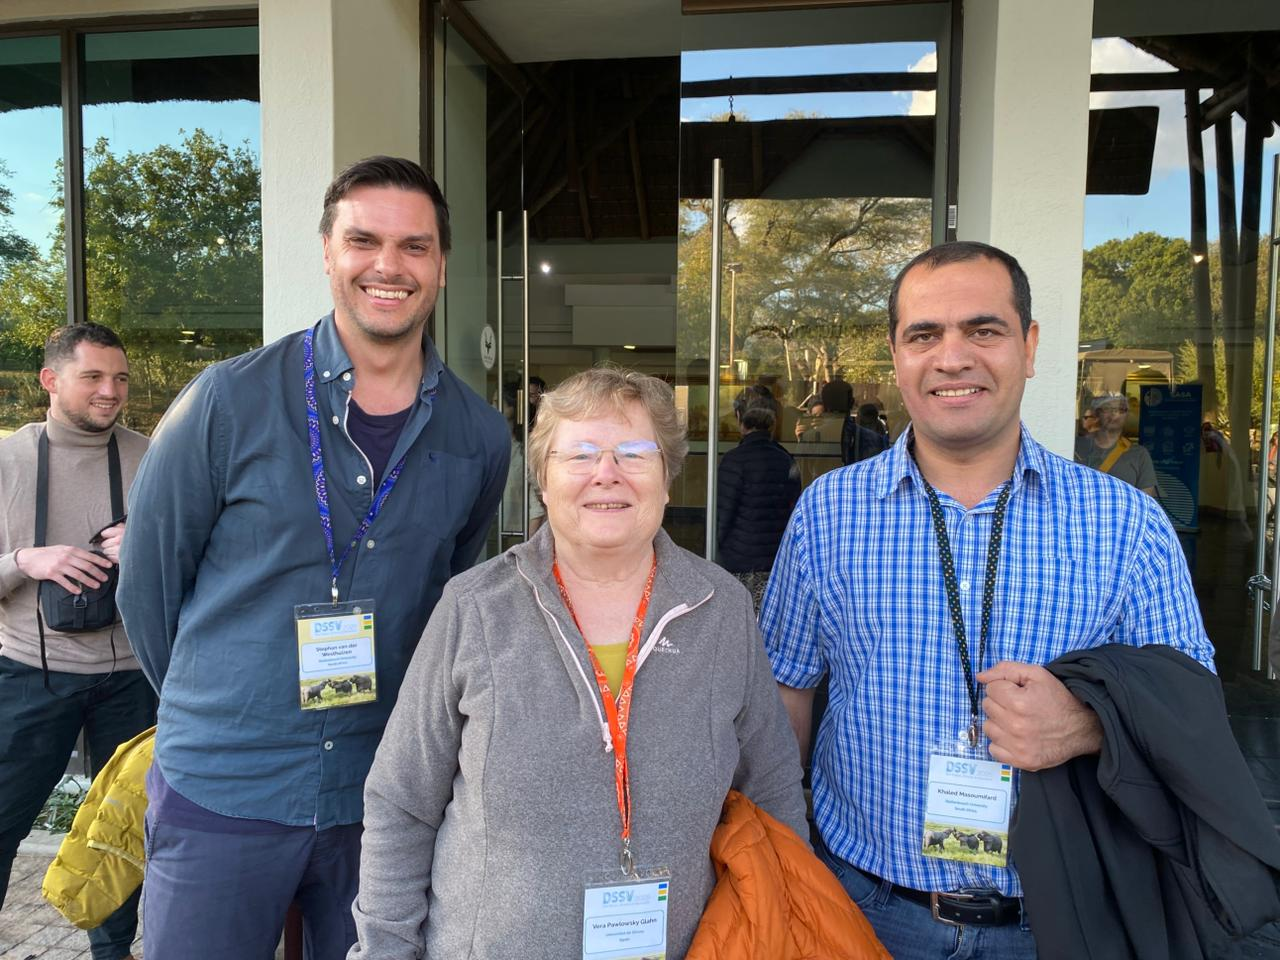
\includegraphics[width=0.4\linewidth]{slides/Vera.jpg}
}
\end{frame}


\begin{frame}{Debates}
\only<1>{
The CoDA school has redefined these principles several times in response to criticism.



        \begin{alertblock}{ (Zier \& Rehder (1998, 2001))}
     They pointed out that even Aitchison’s own earlier work did not strictly satisfy the later CoDA definition of scale invariance.
    \end{alertblock}


        \begin{alertblock}{ (Scealy \& Welsh 2014)}
      The CoDa Principles act as a \textbf{gatekeeping criterion}:
      valid and useful methods have been dismissed simply for not
      conforming to them.
 
      \vspace{0.2cm}
      This is \textbf{unusual, perhaps unique, in statistical
      data analysis}.
    \end{alertblock}
}
\end{frame}



\begin{frame}{One Idea: Transforming to Real Space}





\only<1>{
  \framesubtitle{A transformation $\mathcal{S}^{K-1} \to \mathbb{R}^{K-1}$ unlocks standard inference: regression, PCA, LDA}

  \vspace{0.2cm}
  \renewcommand{\arraystretch}{1.35}
  \setlength{\tabcolsep}{8pt}

  \begin{tabular}{>{\bfseries}l l >{\footnotesize\itshape\color{gray}}l}
    \toprule
    \rowcolor{mainblue}
    \color{white}Method &
    \color{white}Formula &
    \color{white}Reference \\
    \midrule

    \rowcolor{accentblue!20}
    ALR & $\log y_i - \log y_K$ & Aitchison (1982) \\

    \rowcolor{accentblue!20}
    CLR & $\log y_i - K^{-1}\sum_{j=1}^{K} \log y_j$ & Aitchison (1983) \\

    \rowcolor{accentblue!20}
    ILR & $\mathbf{H}\!\left(\log y_i - K^{-1}\sum_{j=1}^{K} \log y_j\right)$ & Egozcue et al.\ (2003) \\

    \midrule
  
    {\normalfont $\alpha$} &
    {\footnotesize $\mathbf{H}[K_\alpha^{-1}(\mathbf{y} \otimes \alpha)]$} &
    Tsagris et al.\ (2011) \\

    {\normalfont BC$_1$} &
    {\footnotesize $\lambda^{-1}\!\left[(y_i / y_K)^\lambda - 1\right]$} &
    Aitchison (2003) \\

    {\normalfont BC$_2$} &
    {\footnotesize $\theta^{-1}(y_i^\theta - 1)$} &
    Greenacre (2010) \\

    {\normalfont Hyper-spherical} &
    {\footnotesize $\arccos\!\left(\dfrac{y_i}{\prod_{j=i+1}^{K} y_j}\right)$} &
    Wang et al.\ (2007) \\

    {\normalfont Square root} &
    {\footnotesize $\sqrt{y_i}$} &
    Stephens (1982) \\

    \bottomrule
  \end{tabular}

  \vspace{0.2cm}
  {\small\textbf{Key:} ALR, CLR, ILR are the most widely used;
  all resolve singularity of $\Sigma_{\mathbf{X}}$ by mapping to unconstrained $\mathbb{R}^{K-1}$.}
}



\end{frame}








\begin{frame}{Machine learning for CoDA}
      \centering
      \vfill
      \textbf{\Large Machine learning for CoDA}
      \vfill
\end{frame}







\begin{frame}{Machine learning: Random Forest}

\begin{itemize}

\item \textbf{Why machine learning?}  
For responses that are compositional: many predictors with complex non-linear patterns that traditional models cannot capture.

\item \textbf{Common approaches}:  
Apply ML models without considering the simplex geometry, or transform data (with log-ratio transformations) to real space (risking distortion and bias).

\item \textbf{Why Random Forests?}  
RFs are flexible and their splitting rules can be easily adapted to respect the simplex structure.

\item PhD of van der Westhuizen (2024) inspired the idea to use tree splitting to account for coDA
\end{itemize}

    
\end{frame}



\begin{frame}{Random Forests framework}
 
\begin{itemize}
   \item[\textcolor{blue}{\large$\blacktriangleright$}]  Given a sample size $n$ and $m$ covariates:
    \[
        \mathbf{X} \in \mathbb{R}^{n \times m} \quad \text{(covariate matrix)}, \qquad
        \mathbf{Y} \in \mathbb{R}^{n \times k} \quad \text{(response matrix)}
    \]
    
  \item[\textcolor{blue}{\large$\blacktriangleright$}]  Each row of \( \mathbf{Y} \) is a compositional vector:
    \[
        Y_{i,j} > 0 \quad \text{for all } i, j, \qquad \sum_{j=1}^k Y_{i,j} = 1
    \]
        
  
     \item[\textcolor{blue}{\large$\blacktriangleright$}] Goal: learn a mapping
    \[
    \mathbf{x} \;\longrightarrow\; \mathbf{y}
    \]
    respecting the simplex geometry
    \vspace{0.8em}

    % \item[\textcolor{blue}{\large$\blacktriangleright$}] Approach: adapt \textbf{random forests} for compositional outputs
    % \vspace{0.8em}

     \item[\textcolor{blue}{\large$\blacktriangleright$}] After training:
    \begin{itemize}
        \item Predict compositional responses for new inputs
        \item Estimate conditional distribution of responses
    \end{itemize}

\end{itemize}
\end{frame}

\begin{frame}{Random Forest: Overview}

A \textbf{Random Forest} is an ensemble of decision trees, each trained on a
bootstrap sample of the data. Key tuning parameters include:

\vspace{0.5em}

\begin{itemize}
    \item \textbf{Number of trees} ($B$): more trees improve stability but increase cost
    \item \textbf{Tree depth} ($d_{\max}$): controls model complexity and overfitting
    \item \textbf{Minimum node size} ($n_{\min}$): minimum observations required to split a node
    \item \textbf{Covariates per split} ($m_{\text{try}}$): number of randomly selected covariates
    considered at each split; typically set to $\sqrt{p}$
\end{itemize}

\end{frame}

\begin{frame}{Random forest: tree}

\centering
\only<1>{

\begin{columns}
    \begin{column}{0.4\linewidth}
    
        \begin{figure}[h]
\centering
\begin{tikzpicture}[
    node distance=0.8cm,
    box/.style={rectangle, draw, minimum width=1.8cm, minimum height=0.8cm, text centered, font=\small},
    dot/.style={circle, fill=black, minimum size=2pt, inner sep=0pt},
    arrow/.style={->, thick}
]
% Main parent node
\node[box] (parent) {$S$=\\$(y_1, y_2, ..., y_n)$};
% Split point (dot in the middle)
\node[dot, below=0.6cm of parent] (split) {};
% Two child nodes
\node[box, below left=0.8cm and 1.2cm of split] (left) {$S_1$};
\node[box, below right=0.8cm and 1.2cm of split] (right) {$S_2$};
% Connections
\draw (parent) -- (split);
\draw (split) -- (left);
\draw (split) -- (right);
% Loss function arrow and equation
\node[right=1.5cm of split, font=\small] (loss) {$\texttt{criteria} = $ ?};
\draw[arrow] (split) -- (loss);
\end{tikzpicture}

\label{fig:decision_tree_split}
\end{figure}



    \end{column}
\begin{column}{0.6\linewidth}
\vspace{1cm}
$\qquad \qquad$A binary decision tree
\vspace

\resizebox{1\linewidth}{!}{%
        \begin{tikzpicture}[
  level/.style={sibling distance=60mm/#1},
  every node/.style={circle, draw, minimum size=8mm, font=\tiny},
  dots/.style={draw=none, font=\large}
]
\node {Root}
  child {
    node {L1}
    child {
      node {L2}
      child {
        node[dots] {$\vdots$}
      }
      child {
        node[dots] {$\vdots$}
      }
    }
    child {
      node {L2}
      child {
        node[dots] {$\vdots$}
      }
      child {
        node[dots] {$\vdots$}
      }
    }
  }
  child {
    node {R1}
    child {
      node {L2}
      child {
        node[dots] {$\vdots$}
      }
      child {
        node[dots] {$\vdots$}
      }
    }
    child {
      node {L2}
      child {
        node[dots] {$\vdots$}
      }
      child {
        node[dots] {$\vdots$}
      }
    }
  };
\end{tikzpicture}}
    \end{column}

    
\end{columns}


}

\end{frame}






\begin{frame}{}\only<1>{\frametitle{MSE splitting}

\begin{tikzpicture}[
  node distance=1cm and 1cm,
  every node/.style={font=\small},
  data/.style={rectangle, draw, align=center, fill=blue!5, rounded corners, inner sep=5pt},
  split/.style={->, thick},
  highlight/.style={->, red, thick, dashed}
  ]
  % Parent node
  \node[data] (parent) {
    \textbf{Parent Node} \\[0.15cm]
    Covariate: $X^{n \times m}$ \\ 
    Response: $Y^{n \times k}$
  };
  % Left child
  \node[data, below left=of parent] (left) {
    \textbf{Left Child} \\[0.1cm]
    Covariate: $X^{n_1 \times m}$ \\
    Response: $Y^{n_1 \times k}$ \\[0.1cm]
    MSE = $\text{MSE}(Y^{n_1 \times k},c,i)$
  };
  % Right child
  \node[data, below right=of parent] (right) {
    \textbf{Right Child} \\[0.1cm]
    Covariate: $X^{n_2 \times m}$ \\
    Response: $Y^{n_2 \times k}$ \\[0.1cm]
    MSE = $\text{MSE}(Y^{n_2 \times k},c,i)$
  };
  % Arrows
  \draw[split] (parent) -- node[midway, left] (leftlabel) {$x_{ij} \leq c$} (left);
  \draw[split] (parent) -- node[midway, right] (rightlabel) {$x_{ij} > c$} (right);
  
  % Optimize labels
  \node[red, left] (opt_i) at ([xshift=-1.5cm, yshift=1.2cm]leftlabel) {\textbf{ } $(c,i)=?$};
  \node[red, right] (opt_c) at ([xshift=1.5cm, yshift=1.2cm]rightlabel) {\textbf{} $(c,i)=?$};
  
  % Short highlight arrows from labels to split conditions
  \draw[highlight] (opt_i) -- (leftlabel.west);
  \draw[highlight] (opt_c) -- (rightlabel.east);
\end{tikzpicture}


}
\only<2>{

\frametitle{Split rule}
\begin{columns}[T]

  \column{0.8\textwidth}
 \begin{center}
\renewcommand{\arraystretch}{1.6}
\begin{tabular}{c|c>{\columncolor{purple!20}}cc>{\columncolor{purple!20}}cc|ccc|c}
\textbf{obs} & $x_1$ & \cellcolor{purple!50}$x_2$ & $x_3$ & \cellcolor{purple!20}$x_4$ & $x_5$ & $y_1$ & $y_2$ & $y_3$ & \textbf{child} \\
\hline
\rowcolor{blue!15}
1 & 0.8 & \textbf{1.2} & 3.4 & 0.5 & 2.1 & 0.60 & 0.25 & 0.15 & \textcolor{blue!80!black}{$\leftarrow$ left} \\
\rowcolor{blue!15}
2 & 2.3 & \textbf{2.7} & 1.1 & 4.2 & 0.9 & 0.10 & 0.70 & 0.20 & \textcolor{blue!80!black}{$\leftarrow$ left} \\
\rowcolor{blue!15}
3 & 1.5 & \textbf{3.1} & 2.9 & 1.8 & 3.3 & 0.45 & 0.45 & 0.10 & \textcolor{blue!80!black}{$\leftarrow$ left} \\
\rowcolor{red!15}
4 & 3.9 & \textbf{4.4} & 0.7 & 3.1 & 1.4 & 0.05 & 0.15 & 0.80 & \textcolor{red!80!black}{right $\rightarrow$} \\
\rowcolor{blue!15}
5 & 0.4 & \textbf{2.0} & 4.5 & 2.7 & 5.0 & 0.50 & 0.30 & 0.20 & \textcolor{blue!80!black}{$\leftarrow$ left} \\
\rowcolor{red!15}
6 & 2.1 & \textbf{5.6} & 3.8 & 0.3 & 2.2 & 0.02 & 0.08 & 0.90 & \textcolor{red!80!black}{right $\rightarrow$} \\
\rowcolor{red!15}
7 & 3.3 & \textbf{3.8} & 1.6 & 4.9 & 0.6 & 0.03 & 0.12 & 0.85 & \textcolor{red!80!black}{right $\rightarrow$} \\
\rowcolor{blue!15}
8 & 1.1 & \textbf{1.5} & 2.2 & 1.1 & 4.4 & 0.55 & 0.35 & 0.10 & \textcolor{blue!80!black}{$\leftarrow$ left} \\
\end{tabular}
\end{center}

  \column{0.22\textwidth}
  \vspace{1em}
  \begin{block}{Partition rule}
    Covariate 2: $i=2$ \\ Split value: $c =3.1$\\
    
  \end{block}
  \vspace{0.8em}
  \textcolor{blue!80!black}{\textbf{Left}} \\
  \hspace{0.5em} $x_2 \leq 3.1$ \\[0.2em]
  \hspace{0.5em} obs: 1, 2, 3, 5, 8 \\[0.6em]
  \textcolor{red!80!black}{\textbf{Right}} \\
   \hspace{0.5em} $x_2 > 3.1$ \\
  \hspace{0.5em} obs: 4, 6, 7


\end{columns}
}


\end{frame}




% %--- SLIDE 1: The data ---
% \begin{frame}{Growing a Tree: The Data}
% \begin{columns}[T]

%   \column{0.65\textwidth}
%   \begin{center}
%   \renewcommand{\arraystretch}{1.6}
%   \begin{tabular}{c|ccccc|ccc}
%   \textbf{obs} & $x_1$ & $x_2$ & $x_3$ & $x_4$ & $x_5$ & $y_1$ & $y_2$ & $y_3$ \\
%   \hline
%   1 & 0.8 & 1.2 & 3.4 & 0.5 & 2.1 & 0.60 & 0.25 & 0.15 \\
%   2 & 2.3 & 2.7 & 1.1 & 4.2 & 0.9 & 0.10 & 0.70 & 0.20 \\
%   3 & 1.5 & 3.1 & 2.9 & 1.8 & 3.3 & 0.45 & 0.45 & 0.10 \\
%   4 & 3.9 & 4.4 & 0.7 & 3.1 & 1.4 & 0.05 & 0.15 & 0.80 \\
%   5 & 0.4 & 2.0 & 4.5 & 2.7 & 5.0 & 0.50 & 0.30 & 0.20 \\
%   6 & 2.1 & 5.6 & 3.8 & 0.3 & 2.2 & 0.02 & 0.08 & 0.90 \\
%   7 & 3.3 & 3.8 & 1.6 & 4.9 & 0.6 & 0.03 & 0.12 & 0.85 \\
%   8 & 1.1 & 1.5 & 2.2 & 1.1 & 4.4 & 0.55 & 0.35 & 0.10 \\
%   \end{tabular}
%   \end{center}

%   \column{0.32\textwidth}
%   \vspace{1em}
%   \begin{block}{Setup}
%     Each node holds $n$ observations with $p$ covariates.
%   \end{block}
%   \vspace{0.8em}
%   \textbf{Response} $\mathbf{y}$ is compositional:
%   \[
%     \mathbf{y} = (y_1, y_2, y_3)
%   \]
%   \[
%     y_k \geq 0, \quad \textstyle\sum_k y_k = 1
%   \]
%   \vspace{0.4em}
%   Lives on the simplex $\mathcal{S}^2$.

% \end{columns}
% \end{frame}


% %--- SLIDE 2: Select covariates ---
% \begin{frame}{Step 1 — Select Covariates}
% \begin{columns}[T]

%   \column{0.65\textwidth}
%   \begin{center}
%   \renewcommand{\arraystretch}{1.6}
%   \begin{tabular}{c|c>{\columncolor{purple!20}}cc>{\columncolor{purple!20}}cc|ccc}
%   \textbf{obs} & $x_1$ & \cellcolor{purple!50}$x_2$ & $x_3$ & \cellcolor{purple!50}$x_4$ & $x_5$ & $y_1$ & $y_2$ & $y_3$ \\
%   \hline
%   1 & 0.8 & 1.2 & 3.4 & 0.5 & 2.1 & 0.60 & 0.25 & 0.15 \\
%   2 & 2.3 & 2.7 & 1.1 & 4.2 & 0.9 & 0.10 & 0.70 & 0.20 \\
%   3 & 1.5 & 3.1 & 2.9 & 1.8 & 3.3 & 0.45 & 0.45 & 0.10 \\
%   4 & 3.9 & 4.4 & 0.7 & 3.1 & 1.4 & 0.05 & 0.15 & 0.80 \\
%   5 & 0.4 & 2.0 & 4.5 & 2.7 & 5.0 & 0.50 & 0.30 & 0.20 \\
%   6 & 2.1 & 5.6 & 3.8 & 0.3 & 2.2 & 0.02 & 0.08 & 0.90 \\
%   7 & 3.3 & 3.8 & 1.6 & 4.9 & 0.6 & 0.03 & 0.12 & 0.85 \\
%   8 & 1.1 & 1.5 & 2.2 & 1.1 & 4.4 & 0.55 & 0.35 & 0.10 \\
%   \end{tabular}
%   \end{center}

%   \column{0.32\textwidth}
%   \vspace{1em}
%   \begin{block}{Random subspace}
%     At each node, draw $m \leq p$ covariates at random.
%   \end{block}
%   \vspace{0.8em}
%   \textcolor{purple!80!black}{\textbf{Selected:}} $x_2,\, x_4$
%   \vspace{0.6em}

%   \begin{itemize}[label={\ding{226}}]
%     \item Reduces correlation between trees
%     \item Only \textcolor{purple!80!black}{highlighted columns} are split candidates
%     \item Other columns are ignored at this node
%   \end{itemize}

% \end{columns}
% \end{frame}


% %--- SLIDE 3: Find the best split ---
% \begin{frame}{Step 2 — Find the Best Split}
% \begin{columns}[T]

%   \column{0.72\textwidth}
%   \begin{center}
%   \renewcommand{\arraystretch}{1.6}
%   \begin{tabular}{c|c>{\columncolor{purple!20}}cc>{\columncolor{purple!20}}cc|ccc|c}
%   \textbf{obs} & $x_1$ & \cellcolor{purple!50}$x_2$ & $x_3$ & \cellcolor{purple!20}$x_4$ & $x_5$ & $y_1$ & $y_2$ & $y_3$ & \\
%   \hline
%   \rowcolor{leftblue}
%   1 & 0.8 & \textbf{1.2} & 3.4 & 0.5 & 2.1 & 0.60 & 0.25 & 0.15 & \textcolor{blue!80!black}{$\leftarrow$ left} \\
%   \rowcolor{leftblue}
%   2 & 2.3 & \textbf{2.7} & 1.1 & 4.2 & 0.9 & 0.10 & 0.70 & 0.20 & \textcolor{blue!80!black}{$\leftarrow$ left} \\
%   \rowcolor{leftblue}
%   3 & 1.5 & \textbf{3.1} & 2.9 & 1.8 & 3.3 & 0.45 & 0.45 & 0.10 & \textcolor{blue!80!black}{$\leftarrow$ left} \\
%   \rowcolor{rightred}
%   4 & 3.9 & \textbf{4.4} & 0.7 & 3.1 & 1.4 & 0.05 & 0.15 & 0.80 & \textcolor{red!80!black}{right $\rightarrow$} \\
%   \rowcolor{leftblue}
%   5 & 0.4 & \textbf{2.0} & 4.5 & 2.7 & 5.0 & 0.50 & 0.30 & 0.20 & \textcolor{blue!80!black}{$\leftarrow$ left} \\
%   \rowcolor{rightred}
%   6 & 2.1 & \textbf{5.6} & 3.8 & 0.3 & 2.2 & 0.02 & 0.08 & 0.90 & \textcolor{red!80!black}{right $\rightarrow$} \\
%   \rowcolor{rightred}
%   7 & 3.3 & \textbf{3.8} & 1.6 & 4.9 & 0.6 & 0.03 & 0.12 & 0.85 & \textcolor{red!80!black}{right $\rightarrow$} \\
%   \rowcolor{leftblue}
%   8 & 1.1 & \textbf{1.5} & 2.2 & 1.1 & 4.4 & 0.55 & 0.35 & 0.10 & \textcolor{blue!80!black}{$\leftarrow$ left} \\
%   \end{tabular}
%   \end{center}

%   \column{0.25\textwidth}
%   \vspace{1em}
%   \begin{block}{Partition rule}
%     \textcolor{purple!80!black}{Best:} $x_2 \leq 3.5$
%   \end{block}
%   \vspace{0.8em}
%   \textcolor{blue!80!black}{\textbf{Left}} \hfill $x_2 \leq 3.5$\\[0.2em]
%   \hspace{0.5em} obs: 1,2,3,5,8 \\[0.6em]
%   \textcolor{red!80!black}{\textbf{Right}} \hfill $x_2 > 3.5$ \\[0.2em]
%   \hspace{0.5em} obs: 4,6,7
%   \vspace{0.6em}



% \end{columns}
% \end{frame}





\begin{frame}{}\only<1>{\frametitle{MSE splitting}

\begin{tikzpicture}[
  node distance=1cm and 1cm,
  every node/.style={font=\small},
  data/.style={rectangle, draw, align=center, fill=blue!5, rounded corners, inner sep=5pt},
  split/.style={->, thick},
  highlight/.style={->, red, thick, dashed}
  ]
  % Parent node
  \node[data] (parent) {
    \textbf{Parent Node} \\[0.15cm]
    Covariate: $X^{n \times m}$ \\ 
    Response: $Y^{n \times k}$
  };
  % Left child
  \node[data, below left=of parent] (left) {
    \textbf{Left Child} \\[0.1cm]
    Covariate: $X^{n_1 \times m}$ \\
    Response: $Y^{n_1 \times k}$ \\[0.1cm]
    MSE = $\text{MSE}(Y^{n_1 \times k},c,i)$
  };
  % Right child
  \node[data, below right=of parent] (right) {
    \textbf{Right Child} \\[0.1cm]
    Covariate: $X^{n_2 \times m}$ \\
    Response: $Y^{n_2 \times k}$ \\[0.1cm]
    MSE = $\text{MSE}(Y^{n_2 \times k},c,i)$
  };
  % Arrows
  \draw[split] (parent) -- node[midway, left] (leftlabel) {$x_{ij} \leq c$} (left);
  \draw[split] (parent) -- node[midway, right] (rightlabel) {$x_{ij} > c$} (right);
  
  % Optimize labels
  \node[red, left] (opt_i) at ([xshift=-1.5cm, yshift=1.2cm]leftlabel) {\textbf{ } $(c,i)=?$};
  \node[red, right] (opt_c) at ([xshift=1.5cm, yshift=1.2cm]rightlabel) {\textbf{} $(c,i)=?$};
  
  % Short highlight arrows from labels to split conditions
  \draw[highlight] (opt_i) -- (leftlabel.west);
  \draw[highlight] (opt_c) -- (rightlabel.east);
\end{tikzpicture}

\begin{align*}
    
(c^*, i^*) 
&=& \operatorname{argmin}_{i,c} \left( \text{MSE}(Y^{n_1 \times k},c,i) + \text{MSE}(Y^{n_2 \times k},c,i) \right)
\\
&=& \arg\min_{c,j} 
\left\{\frac{n_1(c,j)}{n}
\sum_{m=1}^k \sum_{i=1}^{n_1(c,j)} (y_{im}-\bar{y}_{m}^{n_1(c,j)})^2
+
\frac{n_2(c,j)}{n}
\sum_{m=1}^k \sum_{i=1}^{n_2(c,j)} (y_{im}-\bar{y}_{m}^{n_2(c,j)})^2
\right\}.
\end{align*}

}



\only<2>{ \frametitle{MSE splitting}

\begin{tikzpicture}[
  node distance=1cm and 1cm,
  every node/.style={font=\small},
  data/.style={rectangle, draw, align=center, fill=blue!5, rounded corners, inner sep=5pt},
  split/.style={->, thick},
  highlight/.style={->, red, thick, dashed}
  ]
  % Parent node
  \node[data] (parent) {
    \textbf{Parent Node} \\[0.15cm]
    Covariate: $X^{n \times m}$ \\ 
    Response: $Y^{n \times k}$
  };
  % Left child
  \node[data, below left=of parent] (left) {
    \textbf{Left Child} \\[0.1cm]
    Covariate: $X^{n_1 \times m}$ \\
    Response: $Y^{n_1 \times k}$ \\[0.1cm]
    MSE = $\text{MSE}(Y^{n_1 \times k},c,i)$
  };
  % Right child
  \node[data, below right=of parent] (right) {
    \textbf{Right Child} \\[0.1cm]
    Covariate: $X^{n_2 \times m}$ \\
    Response: $Y^{n_2 \times k}$ \\[0.1cm]
    MSE = $\text{MSE}(Y^{n_2 \times k},c,i)$
  };
  % Arrows
  \draw[split] (parent) -- node[midway, left] (leftlabel) {$x_{ij} \leq c$} (left);
  \draw[split] (parent) -- node[midway, right] (rightlabel) {$x_{ij} > c$} (right);
  
  % Optimize labels
  \node[red, left] (opt_i) at ([xshift=-1.5cm, yshift=1.2cm]leftlabel) {\textbf{ } $(c,i)=?$};
  \node[red, right] (opt_c) at ([xshift=1.5cm, yshift=1.2cm]rightlabel) {\textbf{} $(c,i)=?$};
  
  % Short highlight arrows from labels to split conditions
  \draw[highlight] (opt_i) -- (leftlabel.west);
  \draw[highlight] (opt_c) -- (rightlabel.east);
\end{tikzpicture}
\begin{itemize}
    \item 
MSE does not account for the simplex constraint.

\item 
\[V(X_i)=\frac{E(X_i)\left(1-E(X_i)\right)}{\alpha_0+1}\]
\end{itemize}

}

\end{frame}







\begin{frame}
\only<1>{
\frametitle{Dirichlet distribution}


\vspace{1em}

\begin{center}
\colorbox{green!10}{\parbox{0.95\textwidth}{
\begin{center}
\resizebox{\linewidth}{!}{%
\[
    f_{\mathbf{Z}}((z_1,\ldots,z_k); \boldsymbol{\alpha}) = \frac{\Gamma( \alpha_0)}{\prod_{i=1}^k \Gamma(\alpha_i)} \prod_{i=1}^k z_i^{\alpha_i - 1},
\quad  z_i \in [0, 1], \quad \sum_{i=1}^k z_i = 1,
\]
}
\end{center}
}}
\end{center}

\vspace{1.5em}

\begin{itemize}[itemsep=0.8em]


\item[\textcolor{blue}{\large$\blacktriangleright$}] The sum-constant requirement of the simplex is satisfied under the Dirichlet distribution.

\item[\textcolor{blue}{\large$\blacktriangleright$}] \textbf{Extensions available:} Zero-inflated Dirichlet and Kummer–Dirichlet
\end{itemize}
}

\end{frame}


\begin{frame}
\only<1>{\frametitle{Dirichlet log-likelihood splitting}

\begin{tikzpicture}[
  node distance=1cm and 1cm,
  every node/.style={font=\small},
  data/.style={rectangle, draw, align=center, fill=blue!5, rounded corners, inner sep=5pt},
  split/.style={->, thick},
  highlight/.style={->, red, thick, dashed}
  ]
  % Parent node
  \node[data] (parent) {
    \textbf{Parent Node} \\[0.15cm]
    Covariate: $X^{n \times m}$ \\ 
    Response: $Y^{n \times k}$
  };
  % Left child
  \node[data, below left=of parent] (left) {
    \textbf{Left Child} \\[0.1cm]
    Covariate: $X^{n_1 \times m}$ \\
    Response: $Y^{n_1 \times k}$ \\[0.1cm]
     log-like = $\mathcal{L}(Y^{n_1 \times k},c,i)$
  };
  % Right child
  \node[data, below right=of parent] (right) {
    \textbf{Right Child} \\[0.1cm]
    Covariate: $X^{n_2 \times m}$ \\
    Response: $Y^{n_2 \times k}$ \\[0.1cm]
     log-like = $\mathcal{L}(Y^{n_2 \times k},c,i)$
  };
  % Arrows
  \draw[split] (parent) -- node[midway, left] (leftlabel) {$X_{i} \leq c$} (left);
  \draw[split] (parent) -- node[midway, right] (rightlabel) {$X_{i} > c$} (right);
  
  % Optimize labels
  \node[red, left] (opt_i) at ([xshift=-1.5cm, yshift=1.2cm]leftlabel) {\textbf{ } $(c,i)=?$};
  \node[red, right] (opt_c) at ([xshift=1.5cm, yshift=1.2cm]rightlabel) {\textbf{} $(c,i)=?$};
  
  % Short highlight arrows from labels to split conditions
  \draw[highlight] (opt_i) -- (leftlabel.west);
  \draw[highlight] (opt_c) -- (rightlabel.east);
\end{tikzpicture}
\[
(c^*, i^*) = \operatorname{argmax}_{i,c} \left( \max_{\boldsymbol{\alpha}} \mathcal{L}(Y^{n_1 \times k},c,i) + \max_{\boldsymbol{\alpha}} \mathcal{L}(Y^{n_2 \times k},c,i) \right)
\]
}
\end{frame}

\begin{frame}{Prediction based on DirichletRF}

    
\begin{columns}[T]

% Left column - Graph
\begin{column}{0.45\textwidth}
\centering
\begin{tikzpicture}[
    node/.style={ellipse, draw, minimum width=1.2cm, minimum height=0.8cm, thick},
    leaf/.style={rectangle, draw, minimum width=1.8cm, minimum height=0.6cm, thick},
    arrow/.style={->, thick, blue},
    scale=0.75,
    every node/.style={transform shape}
]

% Root node
\node[node] (root) at (0,0) {};

% Level 1
\node[node] (n1) at (-2,-2) {};
\node (dots1) at (1,-2) {\vdots};

% Level 2
\node (dots2) at (-3,-3.5) {\vdots};
\node[node] (n2) at (-1,-4) {};

% Level 3
\node (dots3) at (-2.5,-5.5) {\vdots};
\node[node] (n3) at (0,-6) {};

% Level 4
\node (dots4) at (1,-7.5) {\vdots};
\node[leaf] (leaf) at (-1,-8) {$\{y_1, y_2, \ldots, y_{n_t^'}\}$};

% Arrows - traversal path highlighted
\draw[arrow, line width=1.5pt] (root) -- (n1);
\draw[arrow, dashed] (root) -- (dots1);
\draw[arrow, dashed] (n1) -- (dots2);
\draw[arrow, line width=1.5pt] (n1) -- (n2);
\draw[arrow, dashed] (n2) -- (dots3);
\draw[arrow, line width=1.5pt] (n2) -- (n3);
\draw[arrow, line width=1.5pt] (n3) -- (leaf);
\draw[arrow, dashed] (n3) -- (dots4);

\end{tikzpicture}
\end{column}

% Right column - Explanation
\begin{column}{0.52\textwidth}
\small

\textbf{Process:}
\begin{itemize}
\item[1)] Start at root node
    \item[2)] Traverse tree based on decision rules
    \item[3)] Reach terminal node with observations
\end{itemize}

\vspace{0.4cm}

\textbf{Default Approach:}
\begin{itemize}
    \item Mean: $\hat{y} = \frac{1}{n_t^'}\sum_{i=1}^{n_t^{'}} y_i$
    \item Expectation: $\text{E}(Y_i) = \frac{\hat{\alpha}_i}{\sum_{j+1}^k\hat{\alpha}_i}$
    \item Random Forest: average across trees
\end{itemize}

\vspace{0.4cm}

\textbf{Distributional Approach:}
\begin{itemize}
    \item Collect terminal nodes from all trees
    \item Construct empirical probability function
\end{itemize}

\end{column}

\end{columns}

\end{frame}










%-----------------------------------------------------------------------------
%===================================================
% Comparison Results


\begin{frame}{Comparison Results}
      \centering
      \vfill
      \textbf{\Large Comparison Results}
      \vfill
\end{frame}

\begin{frame}{Performance Evaluation and Transformations}

To evaluate DirichletRF's performance, we compare it with two alternative approaches:
\begin{itemize}
    \item[1)] \textbf{ILR-RF:} A Random Forest model based on log-ratio transformations. 
    The compositional data are first transformed into the ILR
    space. Then, a standard Random Forest is applied to the transformed data, and 
    finally, the predictions are mapped back to the simplex for interpretation.

    \item[2)] \textbf{Dirichlet Regression:} A parametric approach that, 
    works directly on the simplex without requiring any transformation.
\end{itemize}

\end{frame}




\begin{frame}{Evaluation Metrics}

To compare these models, we used  the Aitchison Distance.
\vspace{0.2cm}
\[
AC = \frac{1}{n} \sum_{i=1}^n \sqrt{\sum_{j=1}^k \left(\log\frac{Y_{ij}}{g(\mathbf{Y}_i)} - \log\frac{\hat{Y}_{ij}}{g(\hat{\mathbf{Y}}_i)}\right)^2},
\]
\[
\text{where} \quad g(\mathbf{Y}_i) = \left(\prod_{j=1}^k Y_{ij}\right)^{1/k}
\]


\vspace{0.3cm}
\textbf{Interpretation:} Lower values for this metric indicate better predictive accuracy.
\end{frame}








\begin{frame}{}

    \only<1>{
  
    \textbf{Simple structure simulations}: We use a simple dataset with $3$ Covariate variables, $X_1,X_1, X_{3}$ and with a $3$-dimensional response, $(Y_1,\,Y_2,\,Y_3)$ such that $Y_1+Y_2+Y_3 = 1$. The response is assumed to follow a Dirichlet distribution with the following parameters:
\[
\alpha_1 = 1 + 2 X_1,\quad \alpha_2 =1 + 0.5 X_2,\quad \alpha_3 = 1 + X_3.
\]
\[
(Y_1,\,Y_2,\,Y_3)\sim Dirichlet(\alpha_1,\alpha_2,\alpha_3)
\]
    }
    \only<2>{
      
Dirichlet Regression performed better than the other models. This result makes sense, because the data was generated using a Dirichlet distribution with a linear structure.


But, Dirichlet Random Forest does not perform well in this case — in fact, it gives the worst performance in terms of Aitchison Distance and RMSE.
\begin{table}[htbp]
\centering
\small 
\begin{tabular}{|l|l|c|c|}
\hline
$N$ & Model & Aitchison Distance & Train-Test \\
\hline
\multirow{3}{*}{200} 
    & ILR-RF & 1.303 (0.143) & 0.686 \\
    & \textcolor{blue}{Dirichlet Regression} & \textcolor{blue}{\textbf{1.233} (0.139)} & \textcolor{blue}{\textbf{0.030}} \\
    & \texttt{Dirichlet-RF} & 1.451 (0.153) & 0.600 \\
\hline
\multirow{3}{*}{500}
    & ILR-RF & 1.284 (0.077) & 0.685 \\
    & \textcolor{blue}{Dirichlet Regression} & \textcolor{blue}{\textbf{1.234} (0.078)} & \textcolor{blue}{\textbf{0.035}} \\
    & \texttt{Dirichlet-RF} & 1.450 (0.077) & 0.616 \\
\hline
\multirow{3}{*}{2000}
    & ILR-RF & 1.252 (0.032) & 0.654 \\
    & \textcolor{blue}{Dirichlet Regression} & \textcolor{blue}{\textbf{1.209} (0.032)} & \textcolor{blue}{\textbf{0.006}} \\
    & \texttt{Dirichlet-RF} & 1.431 (0.041) & 0.596 \\
\hline
\end{tabular}
\caption{Values represent the means and (standard deviations) of the metrics for test datasets. Train-Test Diff represents the absolute difference between train and test Aitchison Distance, indicating model generalisation capability.}
\label{tab:performance-comparison1}
\end{table}}

    \only<3>{
    	    

    
    Complex structure synthetic simulations: The dataset consisted of 10 predictor variables \((X_1, \ldots, X_{10})\), with only the first three variables \((X_1, X_2, X_3)\) being truly informative for predicting the compositional response. The three-component compositional response vector $\mathbf{Y} = (Y_1,Y_2,Y_3)$ was constructed through complex non-linear transformations of the informative Covariates. }
    \end{frame}
\begin{frame}
    \only<1>{

\begin{columns}
\begin{column}{0.5\linewidth}

% where \( \mathcal{N}(\mu_i, 0.5^2) \) represents a normally distributed random variable with mean \( \mu_i \) and standard deviation \( 0.5 \), and \( \epsilon \) is a small positive constant ensuring non-negativity.  
% The compositional response variables \( Y_1, Y_2, Y_3 \) are then obtained via the normalisation:
We generate the variables \( Z_1, Z_2, Z_3 \) as follows:  
\[
Z_i = \max(\epsilon, \mathcal{N}(\mu_i, 0.5)), \quad 
\]
\[
Y_i = \frac{Z_i}{Z_1 + Z_2 + Z_3}, \quad  i = 1,2,3.
\]
% This transformation ensures that \( (Y_1, Y_2, Y_3) \) lies within the unit simplex, preserving the compositional structure of the data.
\end{column}
		\begin{column}{0.5\linewidth}

\begin{align*}
\mu_{1j} &= g(2(1 + \sin(x_{1j}))+x_{2j}^3) \\
\mu_{2j} &= g(1 + 2.5\exp(x_{3j})+x_{1j}^2) \\
\mu_{3j} &= g(1 + (1+x_{2j})^2+x_{3j}^4)
\end{align*}

\end{column}

\end{columns}

Where
\[
g(x_{ij}) =
\begin{cases} 
    2, & x_{ij} < \text{Quantile}(x_i, 0.3) \\
    3, & \text{Quantile}(x_i, 0.3) \leq x_{ij} <\text{Quantile}(x_i, 0.6) \\
    4, & \text{Quantile}(x, 0.6) \leq x_{ij} \leq \text{Quantile}(x_i, 0.8) \\
    1, & x_i > \text{Quantile}(x_i, 0.8)
\end{cases}
\]

}
\end{frame}
\begin{frame}
\only<1>{

In this complex scenario, the results are reversed. Our Dirichlet-RF is now the best model, and Dirichlet Regression is the worst.
\begin{table}[htbp]
\centering
\small 
\begin{tabular}{|l|l|c|c|}
\hline
$N$ & Model & Aitchison Distance & Train-Test \\
\hline
\multirow{3}{*}{200} 
    & ILR-RF & 0.670 (0.151) & 0.364 \\
    & Dirichlet Regression & 0.826 (0.155) & 0.068 \\
    & \textcolor{blue}{\texttt{Dirichlet-RF}} & \textcolor{blue}{\textbf{0.659} (0.152)} & \textcolor{blue}{0.221} \\
\hline
\multirow{3}{*}{500}
    & ILR-RF & 0.618 (0.072) & 0.334 \\
    & Dirichlet Regression & 0.790 (0.075) & 0.029 \\
    & \textcolor{blue}{\texttt{Dirichlet-RF}} & \textcolor{blue}{\textbf{0.606} (0.068)} & \textcolor{blue}{0.201} \\
\hline
\multirow{3}{*}{2000}
    & ILR-RF & 0.557 (0.044) & 0.301 \\
    & Dirichlet Regression & 0.785 (0.044) & 0.016 \\
    & \textcolor{blue}{\texttt{Dirichlet-RF}} & \textcolor{blue}{\textbf{0.544} (0.044)} & \textcolor{blue}{0.178} \\
\hline
\end{tabular}
\caption{Train-Test Diff represents the absolute difference between train and test Aitchison Distance.}
\label{tab:performance-comparison}
\end{table}
}
\end{frame}



\begin{frame}{Learning Curve}
\only<1>{


\begin{figure}
    \centering
    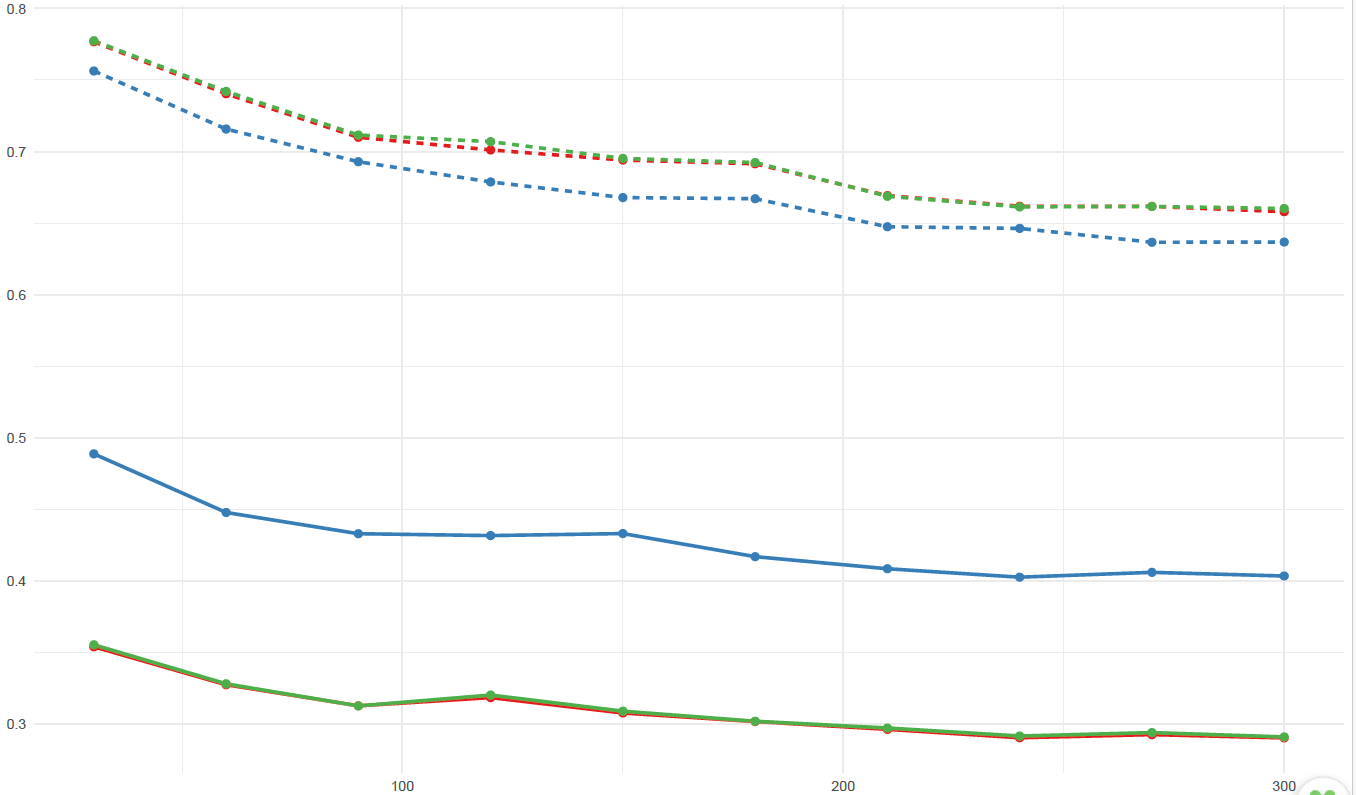
\includegraphics[width=0.75\linewidth]{Learning_curve.png}
    \caption{Aitchison distance as a function of training sample size for all three 
    Random Forest models.}
    \label{fig:enter-label}
\end{figure}
}
\end{frame}




% \begin{frame}
% \only<1>{
% \note{I am not sure to include this slide:

% And for further evaluation of \texttt{Dirichlet-RF}, we also looked at its performance in terms of covariate selection.

% Here, you can see how often each covariate was selected for splitting across all trees, and how much, on average, it contributed to increasing the log-likelihood.

% As I mentioned earlier, only three of the variables were informative — and \texttt{Dirichlet-RF} was able to clearly identify them with high importance.}
% \begin{table}[htbp]
% \centering
% \begin{tabular}{|c|c|c|}
% \hline
% \textbf{Covariate} & \small{Log-Likelihood Importance} & \small{Frequency-Based Importance} \\
% \hline
% \textcolor{blue}{$X_1$} & \textcolor{blue}{225.039} & \textcolor{blue}{14} \\
% \textcolor{blue}{$X_2$} & \textcolor{blue}{303.618} & \textcolor{blue}{21} \\
% \textcolor{blue}{$X_3$} & \textcolor{blue}{272.036} & \textcolor{blue}{19} \\
% \textcolor{red}{$X_4$} & \textcolor{red}{16.839}  & \textcolor{red}{2}  \\
% \textcolor{red}{$X_5$} & \textcolor{red}{9.972}   & \textcolor{red}{2}  \\
% \textcolor{red}{$X_6$} & \textcolor{red}{15.649}  & \textcolor{red}{3}  \\
% \textcolor{red}{$X_7$} & \textcolor{red}{0}   & \textcolor{red}{0}  \\
% \textcolor{red}{$X_8$} & \textcolor{red}{40.240}  & \textcolor{red}{6}  \\
% \textcolor{red}{$X_9$} & \textcolor{red}{5.369}   & \textcolor{red}{1}  \\
% \textcolor{red}{$X_{10}$} & \textcolor{red}{23.295}  & \textcolor{red}{3}  \\
% \hline
% \end{tabular}
% \caption{Variable importance scores based on log-likelihood improvement and selection frequency, averaged across all trees in the \texttt{Dirichlet-RF}.}

% \label{tab:variable-importance}
% \end{table}

% }
% \end{frame}






\begin{frame}{Implementation \& Code Access}
\note{This model was developed in Julia, and the full code is available on GitHub at the link provided.

We chose Julia mainly because of its strong computational performance. Implementing the model directly in R or Python would be much slower.

However, if you're working in R or Python, you can still use the model by calling the Julia functions from those languages.
We've included clear instructions in the repository, especially on how to connect Julia with R.

We're also planning to develop an R package with a C++ backend, which we hope to submit to CRAN, so the model will be even easier for R users to access.}
\vspace{1em}

\begin{itemize}[itemsep=1em]
\item[\textcolor{blue}{\large$\blacktriangleright$}] Model developed in \textbf{Julia} for computational efficiency

\item[\textcolor{blue}{\large$\blacktriangleright$}] Code available on \href{https://github.com/Xaleed/DirichletRandomForestJulia.git}{\textcolor{blue}{\textbf{GitHub}}}:

\textcolor{blue}{\small{https://github.com/Xaleed/DirichletRandomForestJulia.git}}
  \begin{center}

    \qrcode{https://github.com/Xaleed/DirichletRandomForestJulia.git}
 \end{center}



\end{itemize}

\vspace{1.5em}

\end{frame}


\begin{frame}{Alternative to MLE}
    \only<1>{
    \begin{block}{}
        One simple way to address this issue is to use the method of moments (MoM) as an alternative to maximum likelihood estimation (MLE). MoM gives an approximate solution but is much faster to compute.
    \end{block}
     \begin{block}{}
        We can also combine both approaches — instead of using MoM in all nodes, we can selectively apply it only in nodes where we expect its results to be close to MLE. This helps reduce computation while still keeping good accuracy.
    \end{block}
            \resizebox{0.65\linewidth}{!}{%

\begin{table}[htbp]
\centering

\begin{tabular}{|l|c|c|c|c|}
\hline
\multirow{2}{*}{Metric} & \multicolumn{2}{c|}{MLE} & \multicolumn{2}{c|}{MoM} \\
\cline{2-5}
 & (Train) & (Test) & (Train) & (Test) \\
\hline
Aitchison Distance & 0.3901 & 0.7391 & 0.4068 & 0.7457 \\
\hline
\end{tabular}
\end{table}}



}
\end{frame}



% \begin{frame}[plain]
% % \begin{center}
% %    
\includegraphics[width=5cm]{logo.png} % Optional logo
% %    \end{center}
%   \begin{center}
%       \vspace{2cm}

%     {\Huge \textbf{Thank You!} \par}
%     % \vspace{1cm}
%     % {\Large Questions or Comments? \par}
%     \vspace{1cm}
   
    
%     \qrcode{https://github.com/Xaleed/DirichletRandomForestJulia.git}
%    % \texttt{khaledmasoumifard@sun.ac.za}
%   \end{center}
% \end{frame}





